\section{Graphische Darstellung}

Für Funktionen in einer Variablen kennen wir eine praktische graphische Darstellung: den \textbf{Graphen}.

Der Graph ist die Menge aller Punkte \( (x, y) \) in der Koordinatenebene mit der Eigenschaft, dass \( y = f(x) \) ist.

\begin{center}
	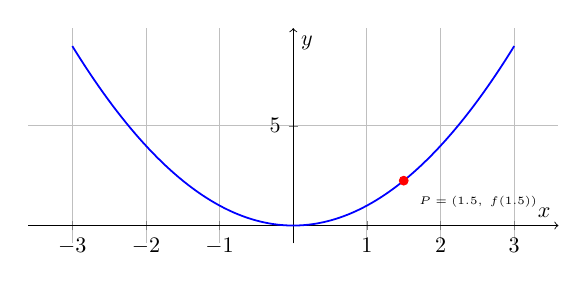
\begin{tikzpicture}[scale = 0.8]
		\begin{axis}[
				axis lines=middle,
				xlabel={$x$},
				ylabel={$y$},
				grid=both,
				domain=-3:3,
				samples=100,
				width=10cm,
				height=5cm,
				axis line style={->},
				enlargelimits=true
			]
			\addplot[blue, thick] {x^2}; % Beispiel: f(x) = x^2

			% Punkt P bei x = 1.5
			\addplot[only marks, mark=*, color=red] coordinates {(1.5, 2.25)};
			\node[color=red, label={below right: \tiny{$P=(1.5,\;f(1.5))$}}] at (axis cs:1.5,2.25) {};
		\end{axis}
	\end{tikzpicture}

\end{center}


Analog lassen sich Funktionen der Form \( f(x, y) \) darstellen. Der Graph ist dann wiederum die Menge aller Punkte \( (x, y, z) \) im dreidimensionalen Raum mit der Eigenschaft, dass \( z = f(x, y) \) ist.
\begin{center}

	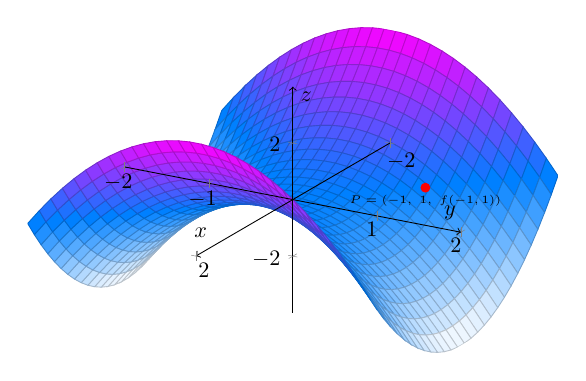
\begin{tikzpicture}[scale = 0.8]
		\begin{axis}[
				view={120}{30},
				xlabel={$x$},
				ylabel={$y$},
				zlabel={$z$},
				domain=-2:2,
				y domain=-2:2,
				samples=30,
				samples y=30,
				axis lines=center,
				axis on top,
				axis line style={->},
				colormap/cool,
				width=10cm,
				height=8cm,
			]
			\addplot3[surf] {x^2 - y^2};
			% Punkt P bei (-1, 1): f(-1,1) = 0
			\addplot3[only marks, mark=*, color=red, mark size=2pt]
			coordinates {(-1, 1, 0)};
			\node[below] at (axis cs:-1,1,0) {\tiny{$P=(-1,\;1,\;f(-1,1))$}};
		\end{axis}
	\end{tikzpicture}
\end{center}
Weil die Koordinatenachsen manchmal die Darstellung stören, werden Sie teilweise in eine Box rund um den Graphen gezeichnet:
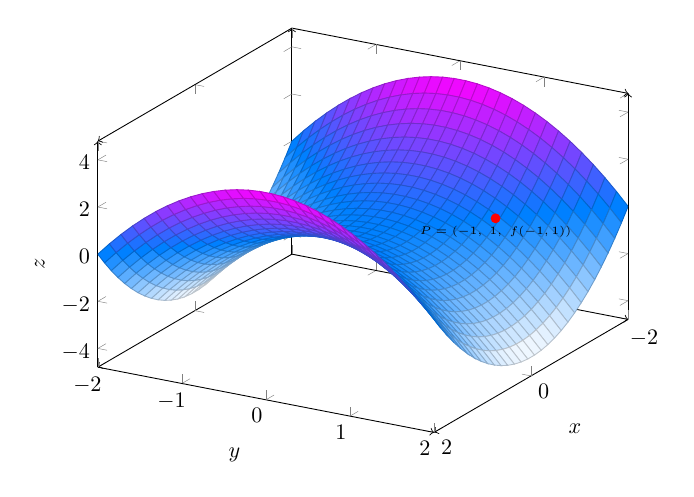
\begin{tikzpicture}[scale = 0.8]
	\begin{axis}[
			view={120}{30},
			xlabel={$x$},
			ylabel={$y$},
			zlabel={$z$},
			domain=-2:2,
			y domain=-2:2,
			samples=30,
			samples y=30,
			% axis lines=center,
			% axis on top,
			axis line style={->},
			colormap/cool,
			width=10cm,
			height=8cm,
		]
		\addplot3[surf] {x^2 - y^2};
		% Punkt P bei (-1, 1): f(-1,1) = 0
		\addplot3[only marks, mark=*, color=red, mark size=2pt]
		coordinates {(-1, 1, 0)};
		\node[below] at (axis cs:-1,1,0) {\tiny{$P=(-1,\;1,\;f(-1,1))$}};
	\end{axis}
\end{tikzpicture}

% \begin{bsp}
% {Der Graph der Funktion $f(x,y)=x^2+ \frac{1}{2} y^2$}{}
% \begin{center}

%     \begin{tikzpicture}
%         \begin{axis}[
%           view={120}{30},
%           xlabel={$x$},
%           ylabel={$y$},
%           zlabel={$z$},
%           domain=-2:2,
%           y domain=-2:2,
%           samples=30,
%           samples y=30,
%         %   axis lines=center,
%         %   axis on top,
%           axis line style={->},
%           colormap/cool,
%           width=10cm,
%           height=8cm,
%         ]
%           \addplot3[surf] {x^2 +0.5* y^2};
%         \end{axis}
%       \end{tikzpicture}
%     \end{center}
% \end{bsp}
% \begin{bsp}
%     {Der Graph der Funktion $f(x,y)=-xy$}{}
%     \begin{center}

%         \begin{tikzpicture}
%             \begin{axis}[
%               view={120}{15},
%               xlabel={$x$},
%               ylabel={$y$},
%               zlabel={$z$},
%               domain=-2:2,
%               y domain=-2:2,
%               samples=30,
%               samples y=30,
%             %   axis lines=center,
%             %   axis on top,
%               axis line style={->},
%               colormap/cool,
%               width=10cm,
%               height=8cm,
%             ]
%               \addplot3[surf] {-x*y};
%             \end{axis}
%           \end{tikzpicture}
%         \end{center}
% \end{bsp}
% \begin{bsp}
%     {Der Graph der Funktion $f(x,y)=\sqrt{4-x^2-y^2}$}{}
%     \begin{center}

%         \begin{tikzpicture}
%             \begin{axis}[
%               view={130}{15},
%               xlabel={$x$},
%               ylabel={$y$},
%               zlabel={$z$},
%               %axis lines=center,
%               axis line style={->},
%               ticks=none,
%               samples=40,
%               samples y=30,
%               width=10cm,
%               height=8cm,
%               colormap/cool,
%             ]
%               % Parametrische Darstellung der oberen Halbkugel (r = 2)
%               \addplot3[
%                 surf,
%                 domain=0:90,
%                 y domain=130:490,
%                 variable=\t,
%                 variable y=\p,
%               ]
%               (
%                 {2*sin(\t)*cos(\p)},
%                 {2*sin(\t)*sin(\p)},
%                 {2*cos(\t)}
%               );
%             \end{axis}
%           \end{tikzpicture}
%         \end{center}
% \end{bsp}


Eine Möglichkeit zur Veranschaulichung solcher Graphen besteht darin, \textbf{vertikale Schnitte} des Graphen zu betrachten.
Genauer: Wir schneiden den Graphen mit Ebenen, die parallel zur \( xz \)-Ebene oder zur \( yz \)-Ebene verlaufen. Im ersten Fall gilt: \( y = y_0 = \text{konstant} \). Im zweiten Fall gilt: \( x = x_0 = \text{konstant} \)

\begin{definition}
	{Schnittkurven}{}
	Sei \( f : \mathbb{R}^2 \to \mathbb{R},\ (x, y) \mapsto f(x, y) \), eine Funktion in zwei Variablen.

	Für fixiertes \( y_0 \) (bzw. \( x_0 \)) ist die \textbf{Schnittkurve} definiert als der Graph der Funktion
	\[
		x \mapsto f(x, y_0) \quad \text{bzw.} \quad y \mapsto f(x_0, y).
	\]

	Für jedes fixierte \( y_0 \) oder \( x_0 \) gibt es also eine eigene Schnittkurve. Stellen wir mehrere dieser Kurven zusammen, so erhalten wir ein \textbf{Schnittkurvendiagramm}.

\end{definition}
\begin{bsp}
	{Schnittkurvendiagramm der Funktion $V(x,y) = \frac{1}{2}x^2+y^2$}{}
	Wenn wir $x_0$ fixieren erhalten wir lauter quadratische Funktionen $y \mapsto V(x_0, y)$. Deren Graphen sind Parabeln. In der Abbildung sind die Schnittkurven für $x_0=0, \pm1, \pm2$ dargestellt.
	\begin{center}
		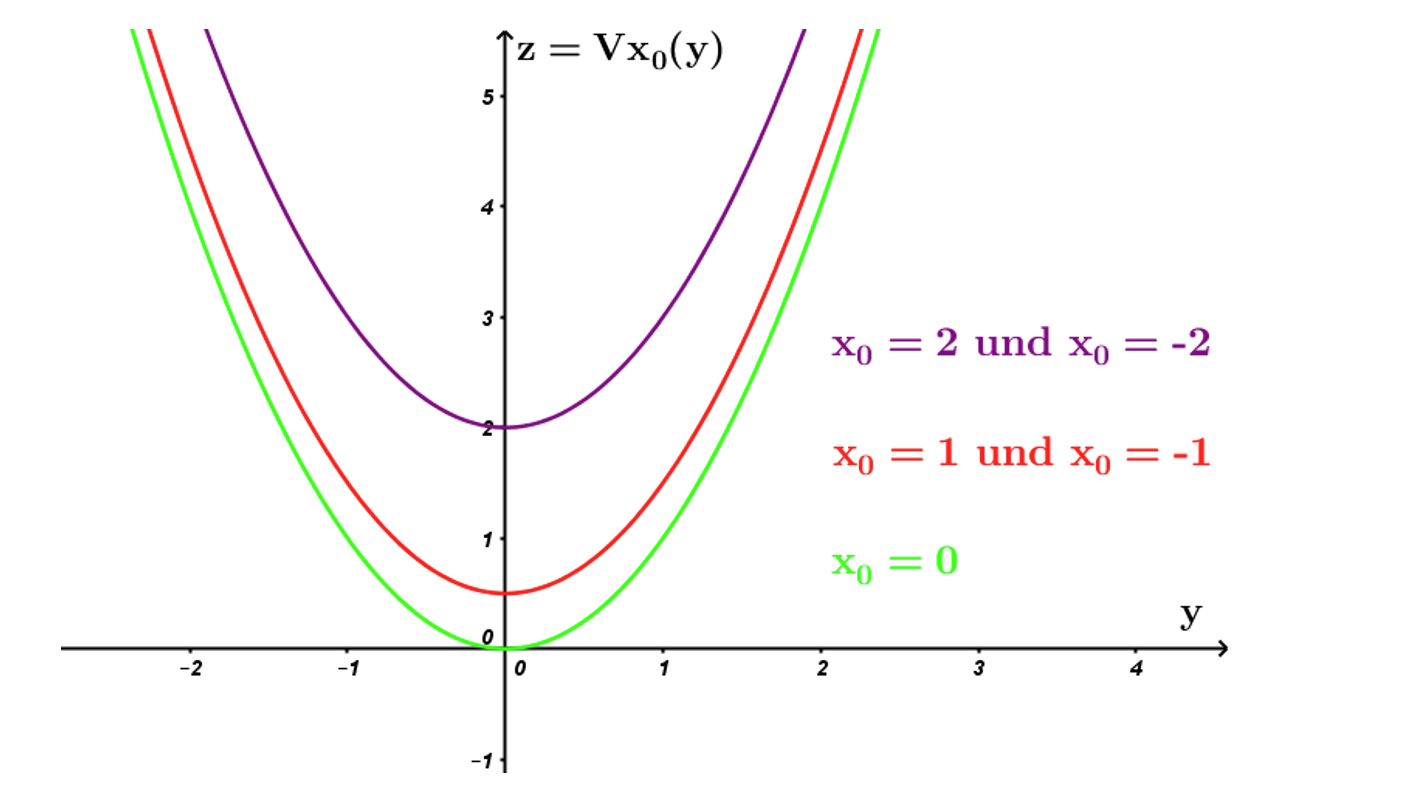
\includegraphics[width = 0.5\textwidth]{media/SchnittkurvenBsp.png}
	\end{center}
	Die gleichen Kurven im Raum platziert:
	\begin{center}
		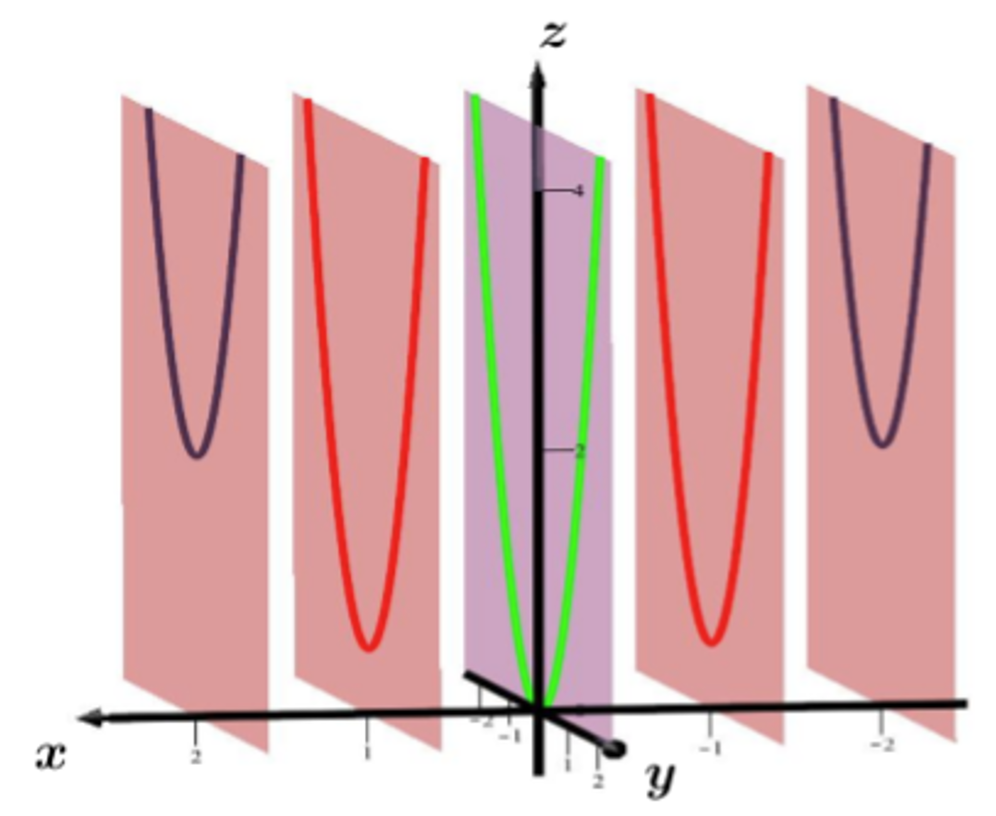
\includegraphics[width = 0.5\textwidth]{media/Schnittkurven-im-Raum.png}
	\end{center}

\end{bsp}
\clearpage
Eine andere Möglichkeit, sich ein Bild von solchen Graphen zu machen sind die \textbf{Niveaulinien}. Dieses Prinzip kennen wir als Höhenlinien auf einer Landkarte.

\begin{definition}
	{Niveaulinien}{}
	Sei \( f : \mathbb{R}^2 \to \mathbb{R},\ (x, y) \mapsto f(x, y) \), eine Funktion in zwei Variablen.

	\textbf{Niveaulinien} von \( f \) bestehen aus allen Inputs, welche auf den gleichen Output führen – das heisst, aus den Lösungen \( (x, y) \) der Gleichung
	\[
		f(x, y) = z_0,
	\]
	wobei \( z_0 \) fixiert, also konstant, ist.

	Niveaulinien sind also Teilmengen der \( xy \)-Ebene, welche auf die gleiche „Höhe“ abgebildet werden.

\end{definition}
% In einigen unserer Beispiele werden die Lösungen solcher Gleichungen \textbf{Kegelschnitte} sein. Hier sind die wichtigsten Formen zusammengestellt:

% \begin{description}
%   \item[Parabeln:] 
%   \[
%   y = ax^2 \quad \text{oder} \quad x = ay^2
%   \]

%   \item[Ellipsen:] 
%   \[
%   \frac{x^2}{a^2} + \frac{y^2}{b^2} = 1
%   \]

%   \item[Hyperbeln:] 
%   \[
%   \frac{x^2}{a^2} - \frac{y^2}{b^2} = 1 \quad \text{oder} \quad -\frac{x^2}{a^2} + \frac{y^2}{b^2} = 1
%   \]
% \end{description}

\begin{bsp}
	{Niveaulinien der Funktion $V(x,y) = \frac{1}{2}x^2+y^2$ }{}
	Für den konstanten Output \( z_0 := c \) ergibt sich:

	\[
		V(x, y) = \frac{x^2}{2} + y^2 = c \iff \frac{x^2}{( \sqrt{2c} )^2} + \frac{y^2}{( \sqrt{c} )^2} = 1
	\]

	Dies sind \textbf{Ellipsen} mit Halbachsenlängen
	\[
		a = \sqrt{2c} \quad \text{und} \quad b = \sqrt{c}.
	\]
	\begin{center}
		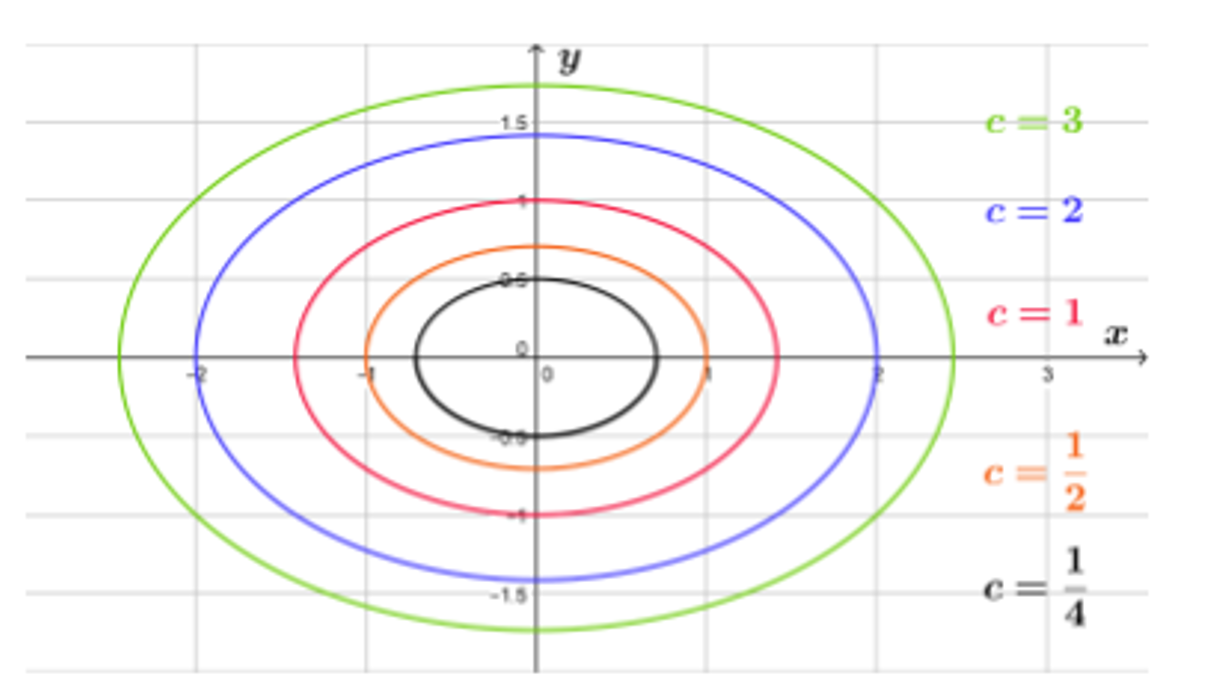
\includegraphics[width = 0.4\textwidth]{media/NiveaulinienBsp.png}
	\end{center}
\end{bsp}

Aus Schnittkurven und Niveaulinien ”verstehen” wir den Graphen von $V$:
\begin{center}
	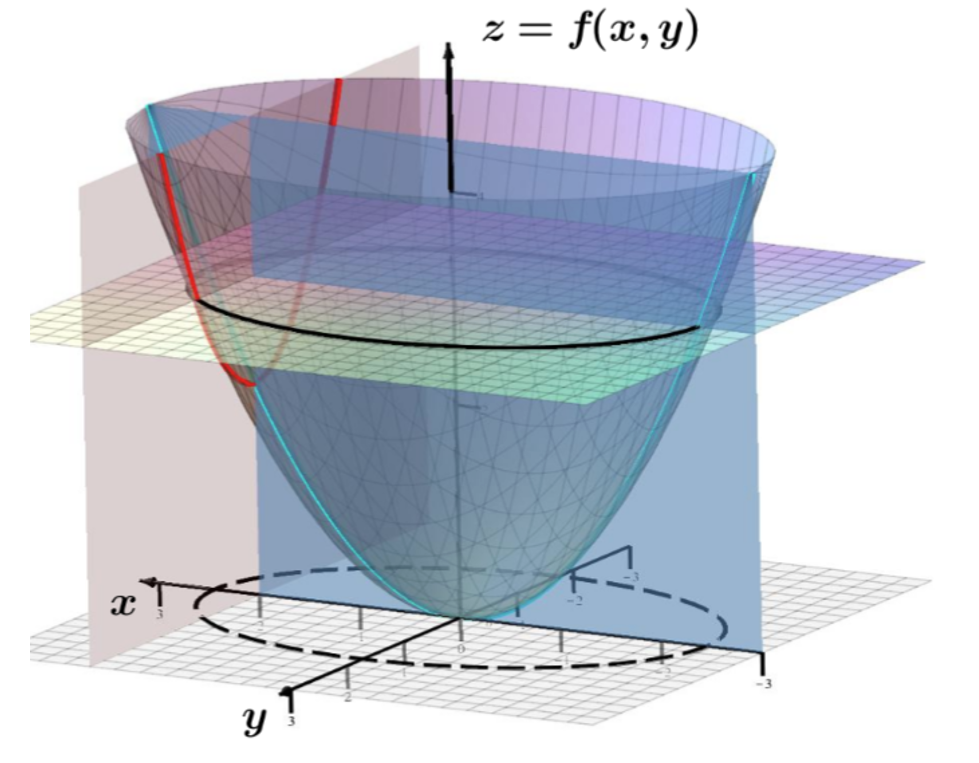
\includegraphics[width = 0.4 \textwidth]{media/GraphAusSchnittkurveNiveaulinien.png}
\end{center}





\begin{ueb}
	{}{}
	\begin{enumerate}
		\item Gegeben ist die Funktion \( f(x, y) = x^2 + 4xy + y^2 - \ln(1 + x^2) \). Prüfen Sie, ob der Punkt \( P = (0, -3) \) auf der Niveaulinie zum Niveau \( z = 9 \) liegt.

		\item Erstellen Sie die Schnittkurvendiagramme der folgenden Funktionen %, bestimmen Sie ihre Niveaulinien 
		      und skizzieren Sie ihre Graphen. Wählen Sie als Schnittkurven die Graphen der Funktionen $x \mapsto f(x, y_0)$ mit $y_0 = -1, 0, 1$
		      \begin{enumerate}
			      %\item \( f(x, y) = \sqrt{x^2 + y^2} \)
			      \item \( f(x, y) = x^2 + 1 \)
			      \item \( f(x, y) = x^2 + y \)
		      \end{enumerate}
		\item Zeichnen Sie das \textbf{Niveaulinienportrait} der folgenden Funktionen. Können Sie sich den Graphen der Funktion damit vorstellen? Überprüfen Sie die Vorstellung, indem Sie den Graphen mit \href{https://www.geogebra.org/calculator}{Geogebra} zeichnen.

		      \begin{enumerate}
			      \item \( f(x, y) = \sqrt{x^2 + y^2} \)
			      \item \( f(x, y) = 2x + 3y \)
			      \item \( g(x, y) = xy \)
		      \end{enumerate}
	\end{enumerate}
\end{ueb}
\clearpage
\emph{Lösungen}
\begin{enumerate}
	\item \begin{align*}
		      f(0, -3)
		       & = (0)^2 + 4 \cdot 0 \cdot (-3) + (-3)^2 - \ln(1 + 0^2) \\
		       & = 0 + 0 + 9 - \ln(1)                                   \\
		       & = 9 - 0                                                \\
		       & = 9
	      \end{align*}

	      Da \( f(0, -3) = 9 \), liegt der Punkt \( P = (0, -3) \) tatsächlich auf der Niveaulinie zum Niveau \( z = 9 \).
	\item Schnittkurvendiagramme:
	      \begin{enumerate}
		      \item \( f(x, y) = x^2 + 1 \)

		            \begin{figure}[h!]
			            \centering
			            \begin{subfigure}[t]{0.48\textwidth}
				            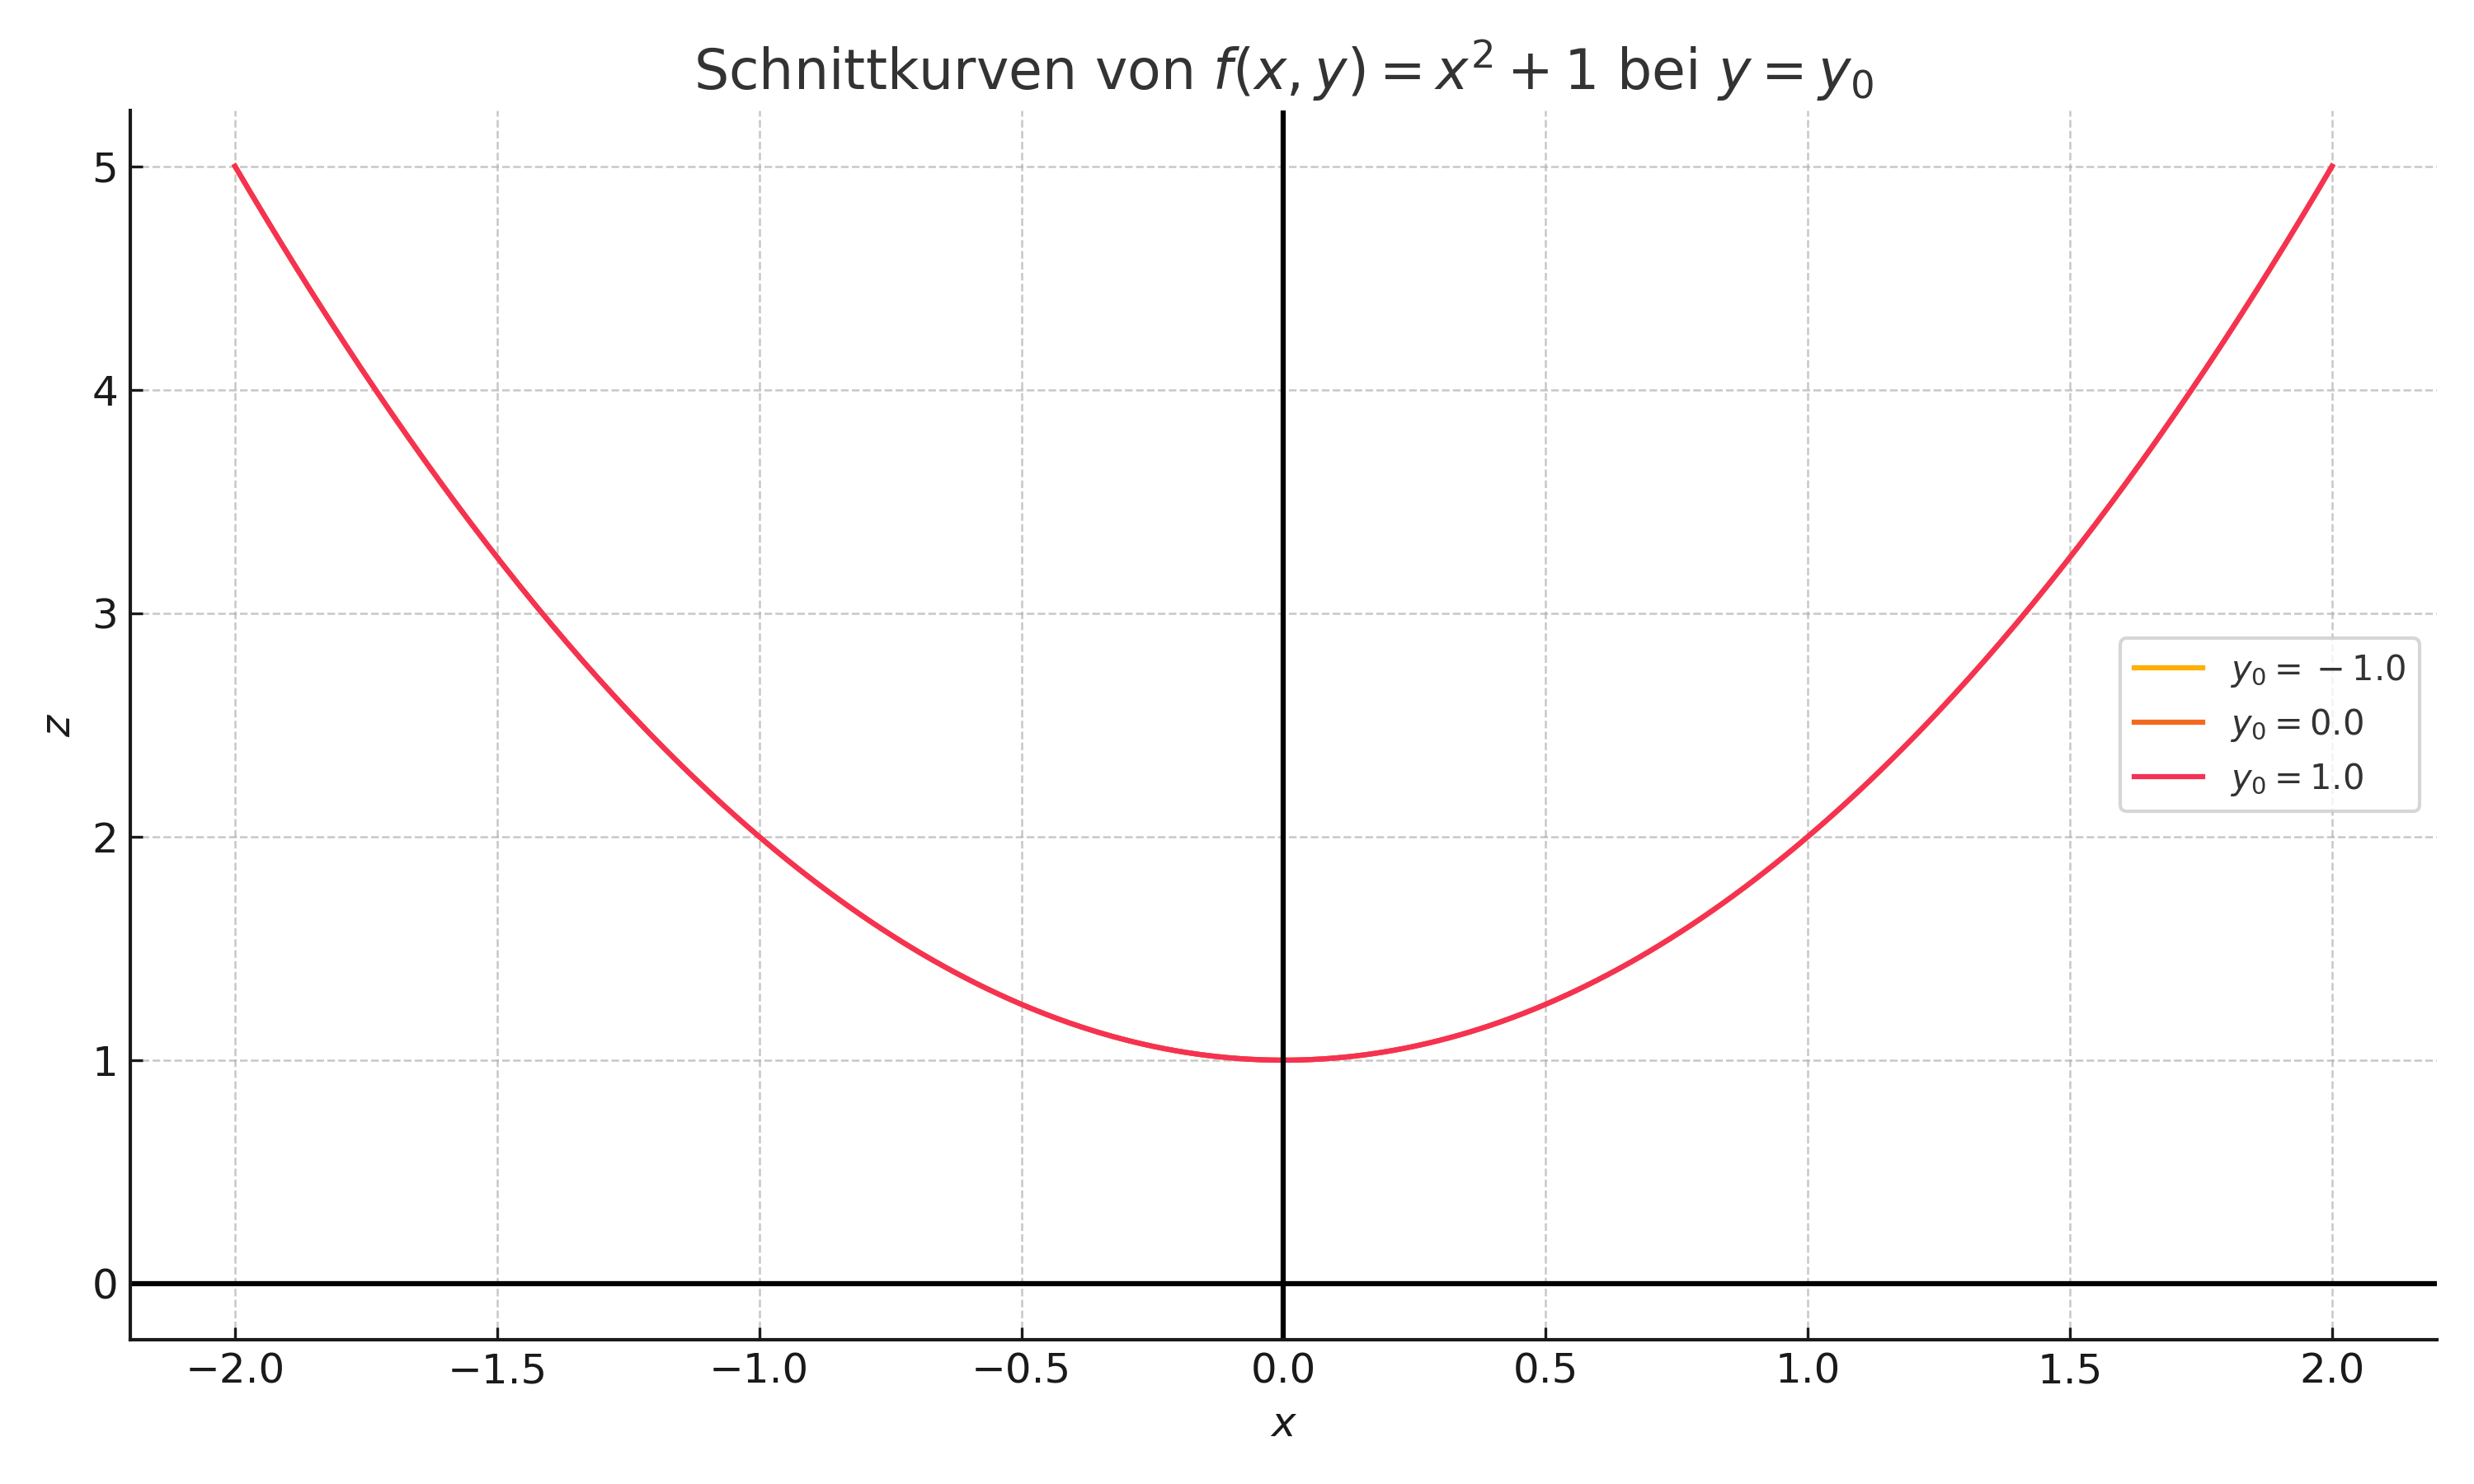
\includegraphics[width=\linewidth]{media/ueb1/schnitt_f1_labeled.png}
				            \caption*{Schnittkurven bei festen \( y_0 \)}
			            \end{subfigure}
			            \hfill
			            \begin{subfigure}[t]{0.48\textwidth}
				            \centering
				            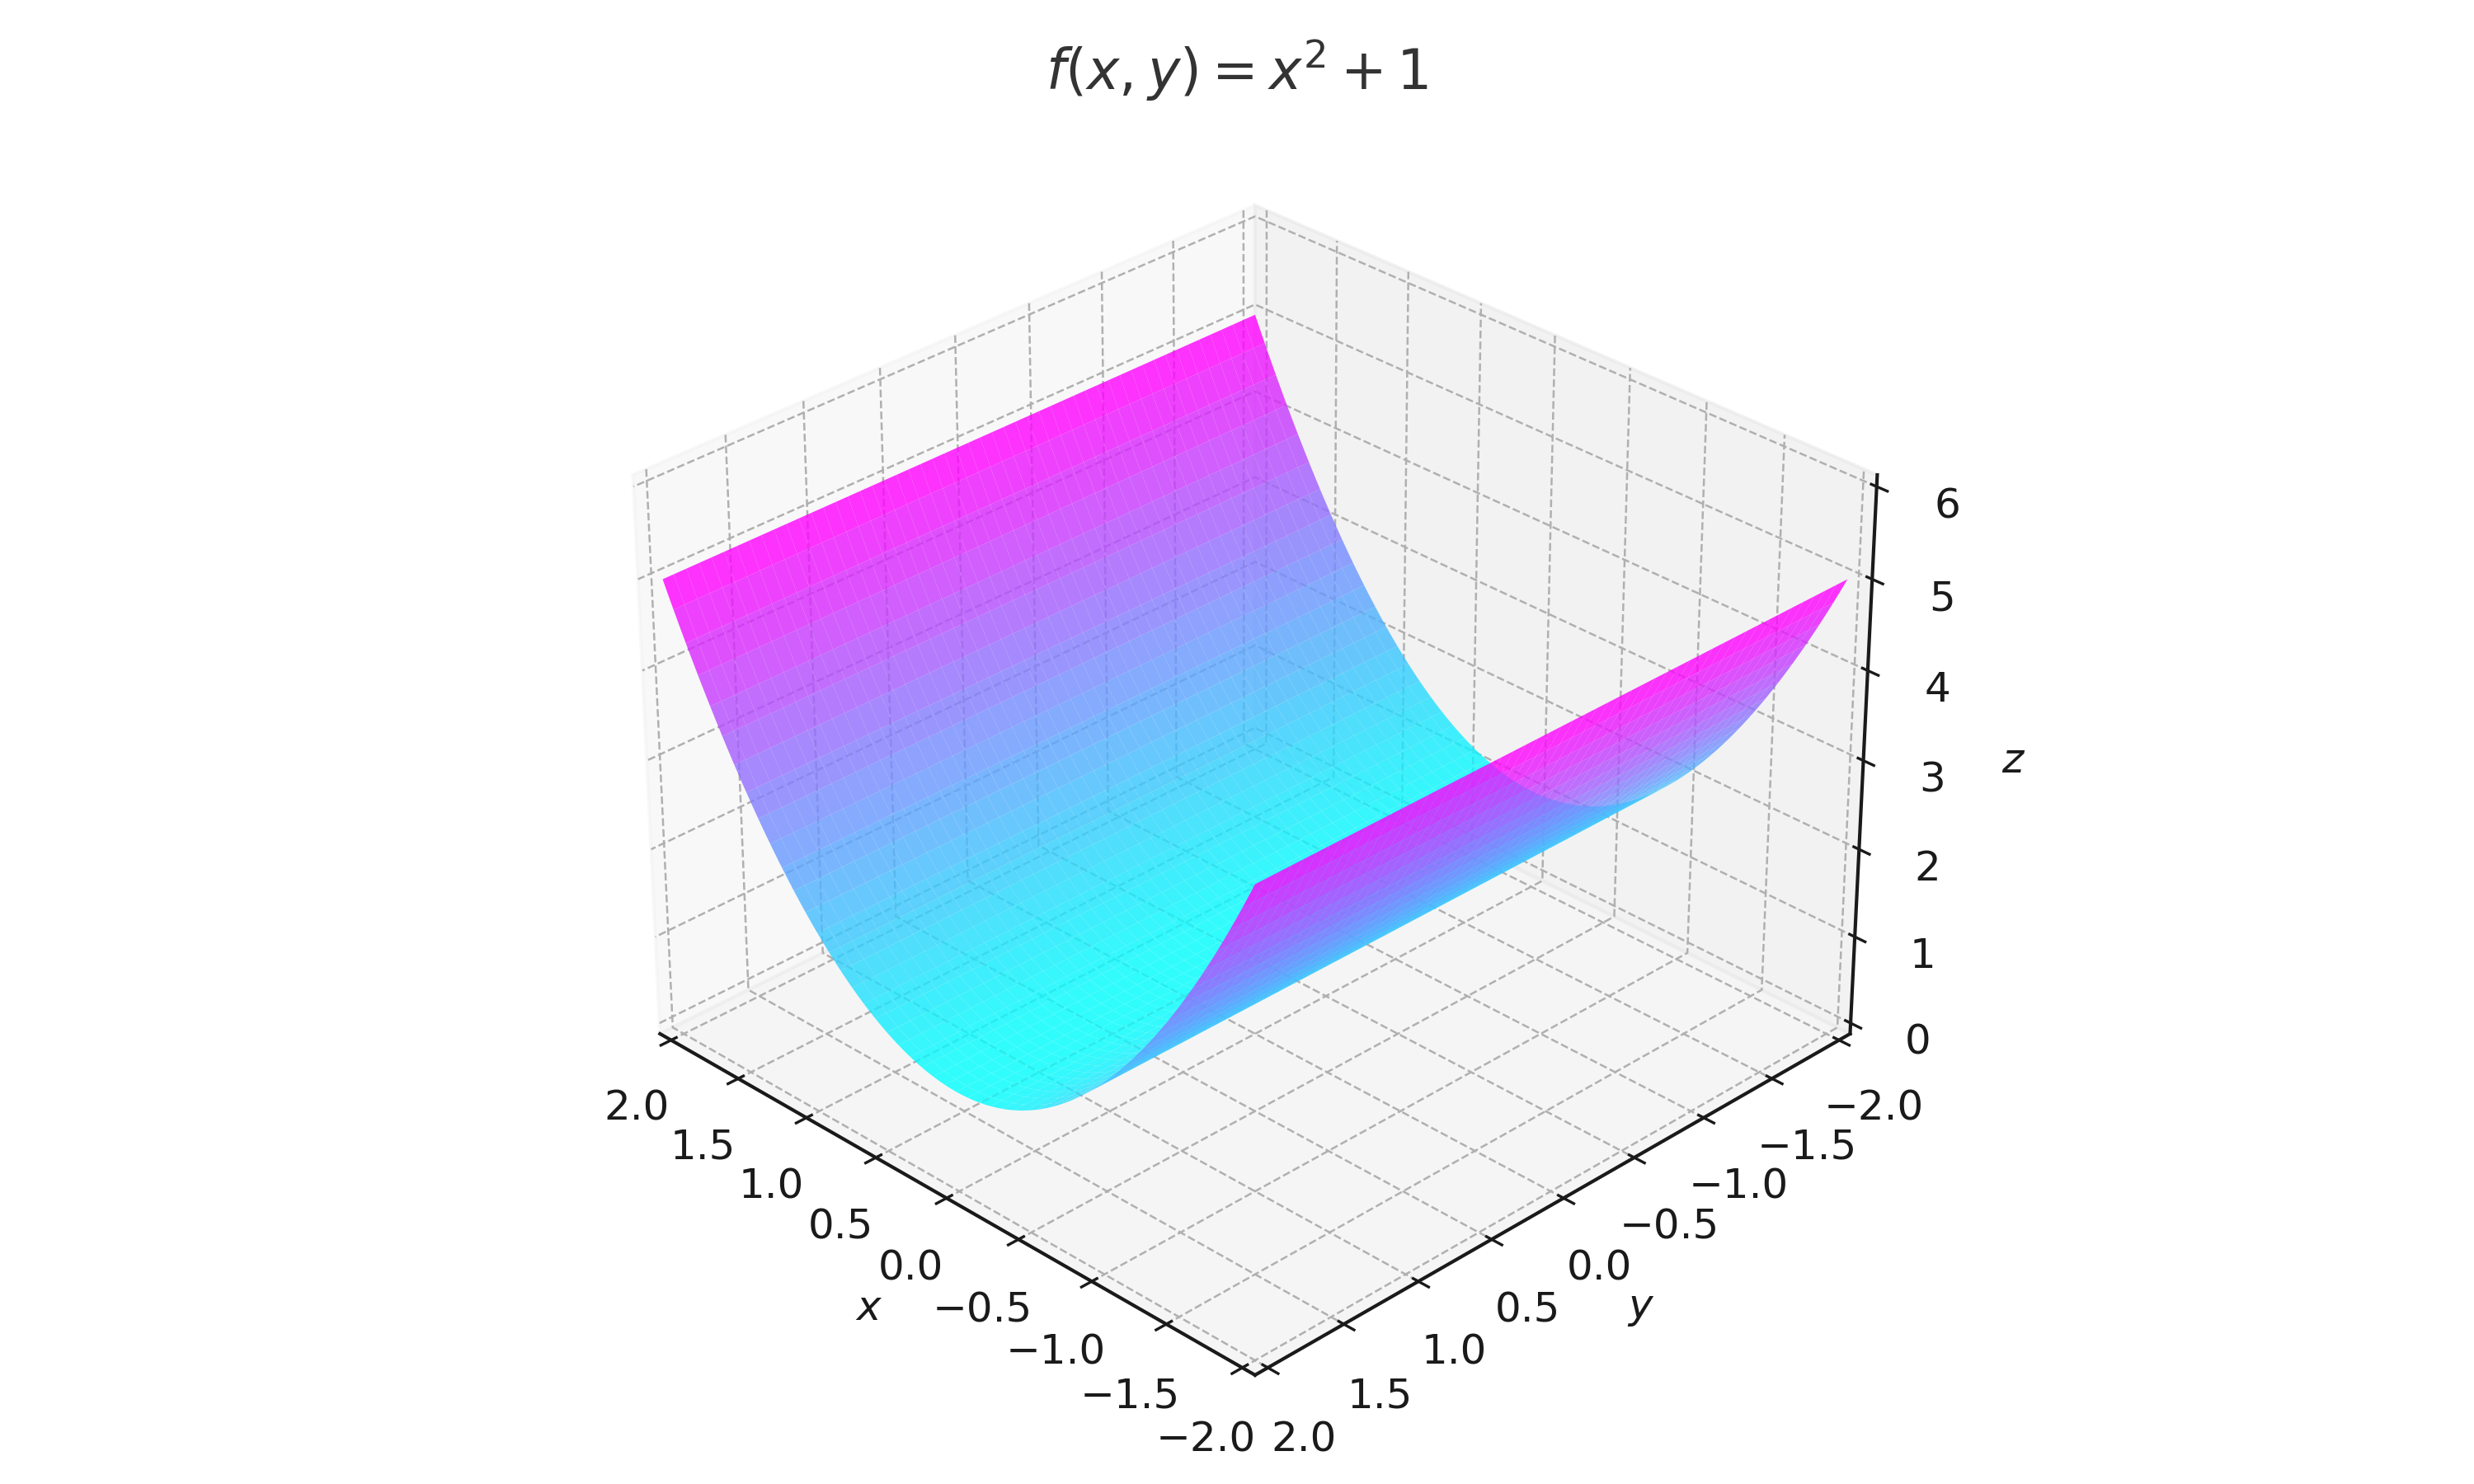
\includegraphics[width=\linewidth]{media/ueb1/graph_f1_labeled.png}
				            \caption*{Graph der Funktion \( f(x, y) \)}
			            \end{subfigure}
			            \caption{Visualisierung von \( f(x, y) = x^2 + 1 \)}
			            % \begin{subfigure}[t]{0.48\textwidth}
			            %   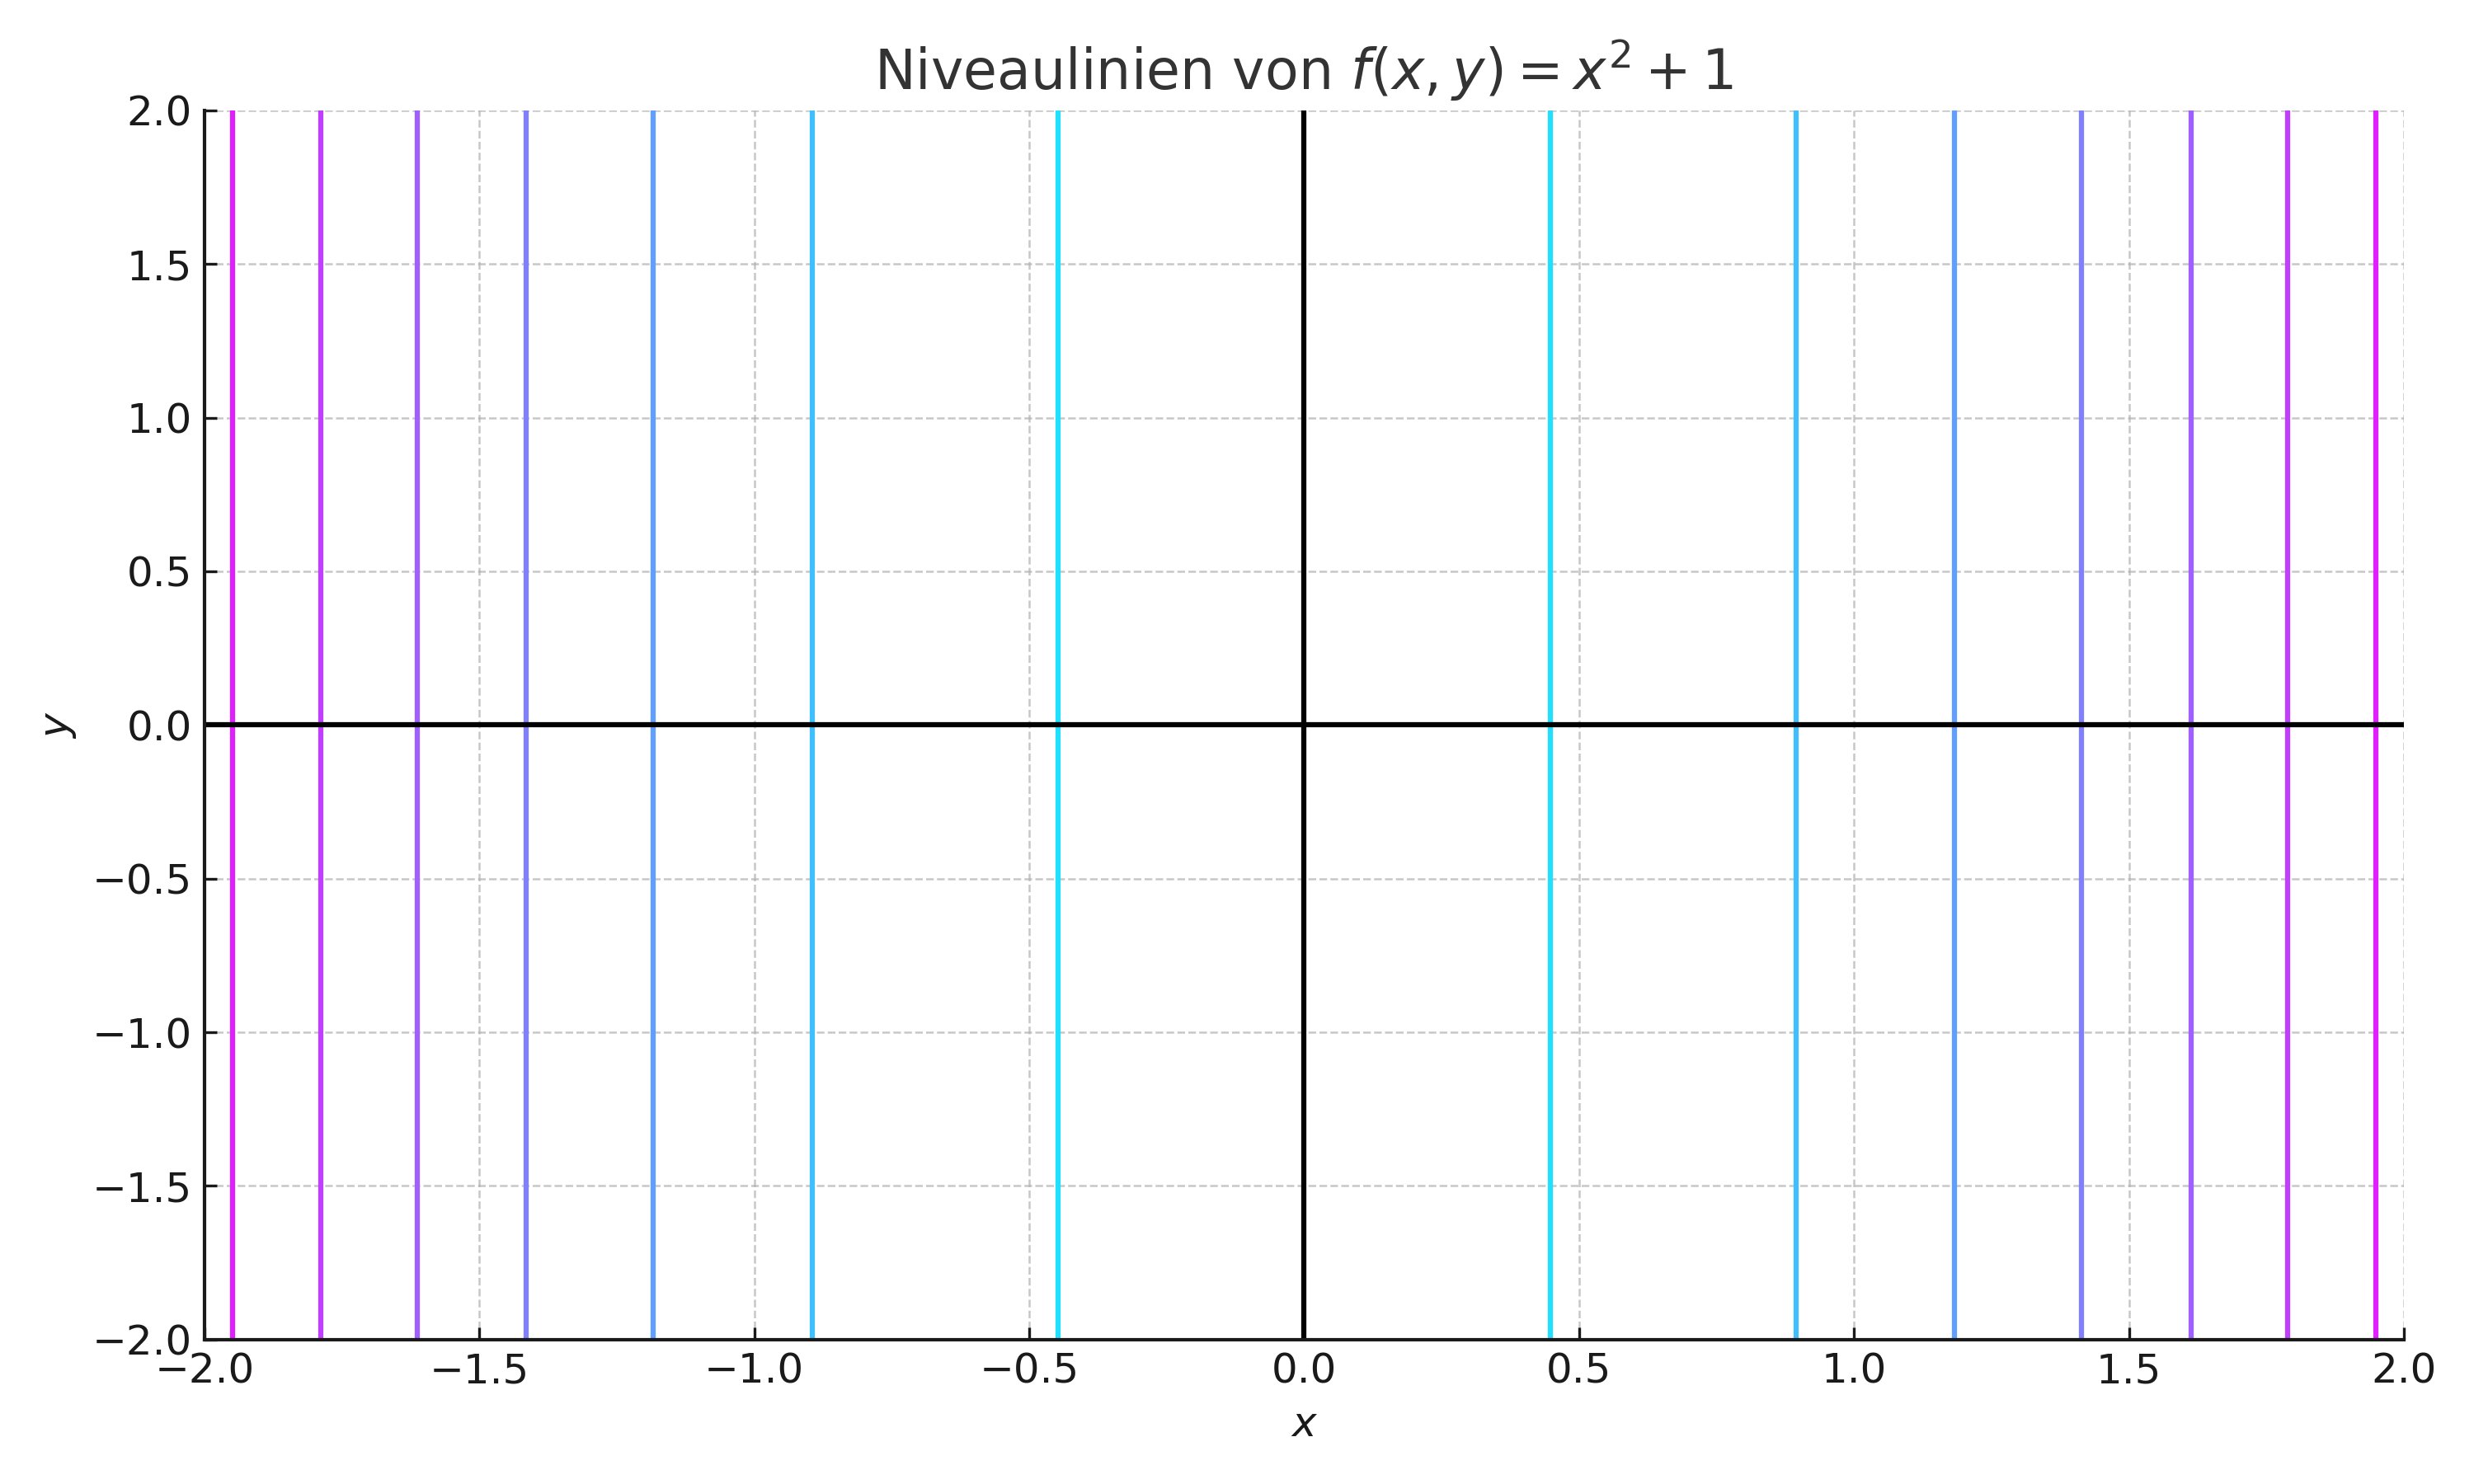
\includegraphics[width=\linewidth]{media/ueb1/niveau_f1_labeled.png}
			            %   \caption{Niveaulinien in der \( xy \)-Ebene}
			            % \end{subfigure}

			            % \vspace{1em}

		            \end{figure}
		      \item \( f(x, y) = x^2 + y \)

		            \begin{figure}[h!]
			            \centering
			            \begin{subfigure}[t]{0.48\textwidth}
				            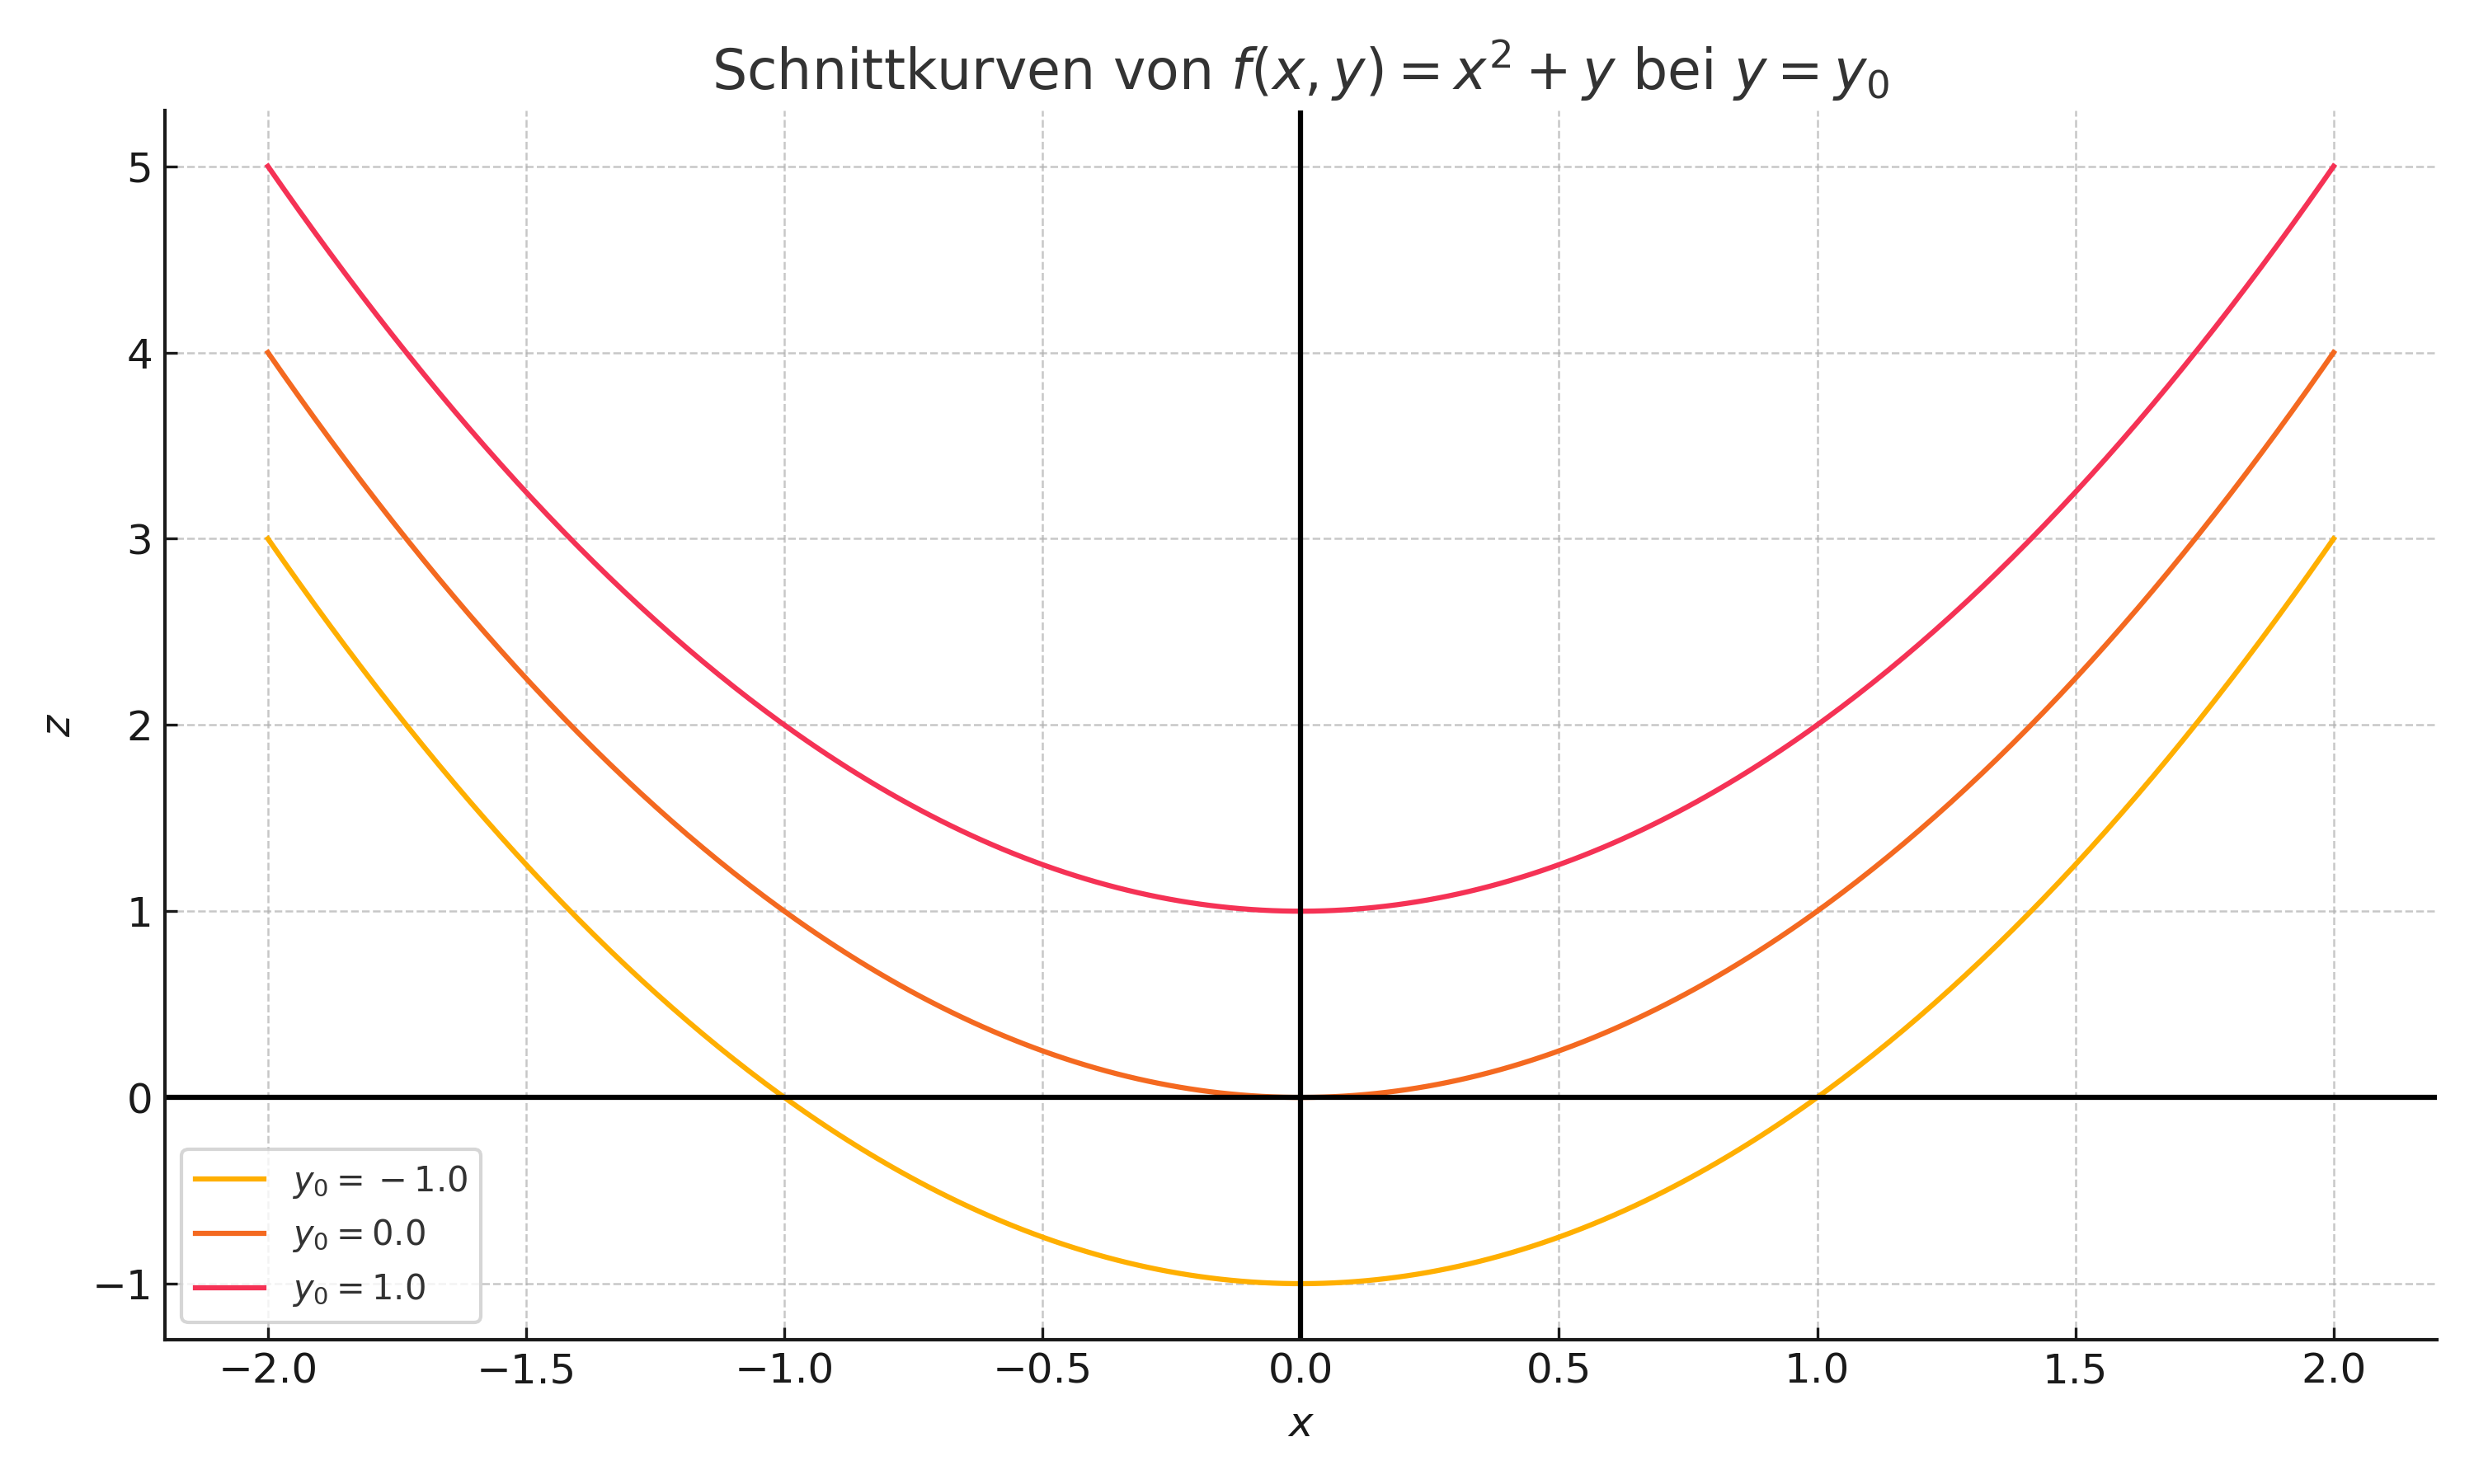
\includegraphics[width=\linewidth]{media/ueb1/schnitt_f2_labeled.png}
				            \caption*{Schnittkurven bei festen \( y_0 \)}
			            \end{subfigure}
			            \hfill
			            \begin{subfigure}[t]{0.48\textwidth}
				            \centering
				            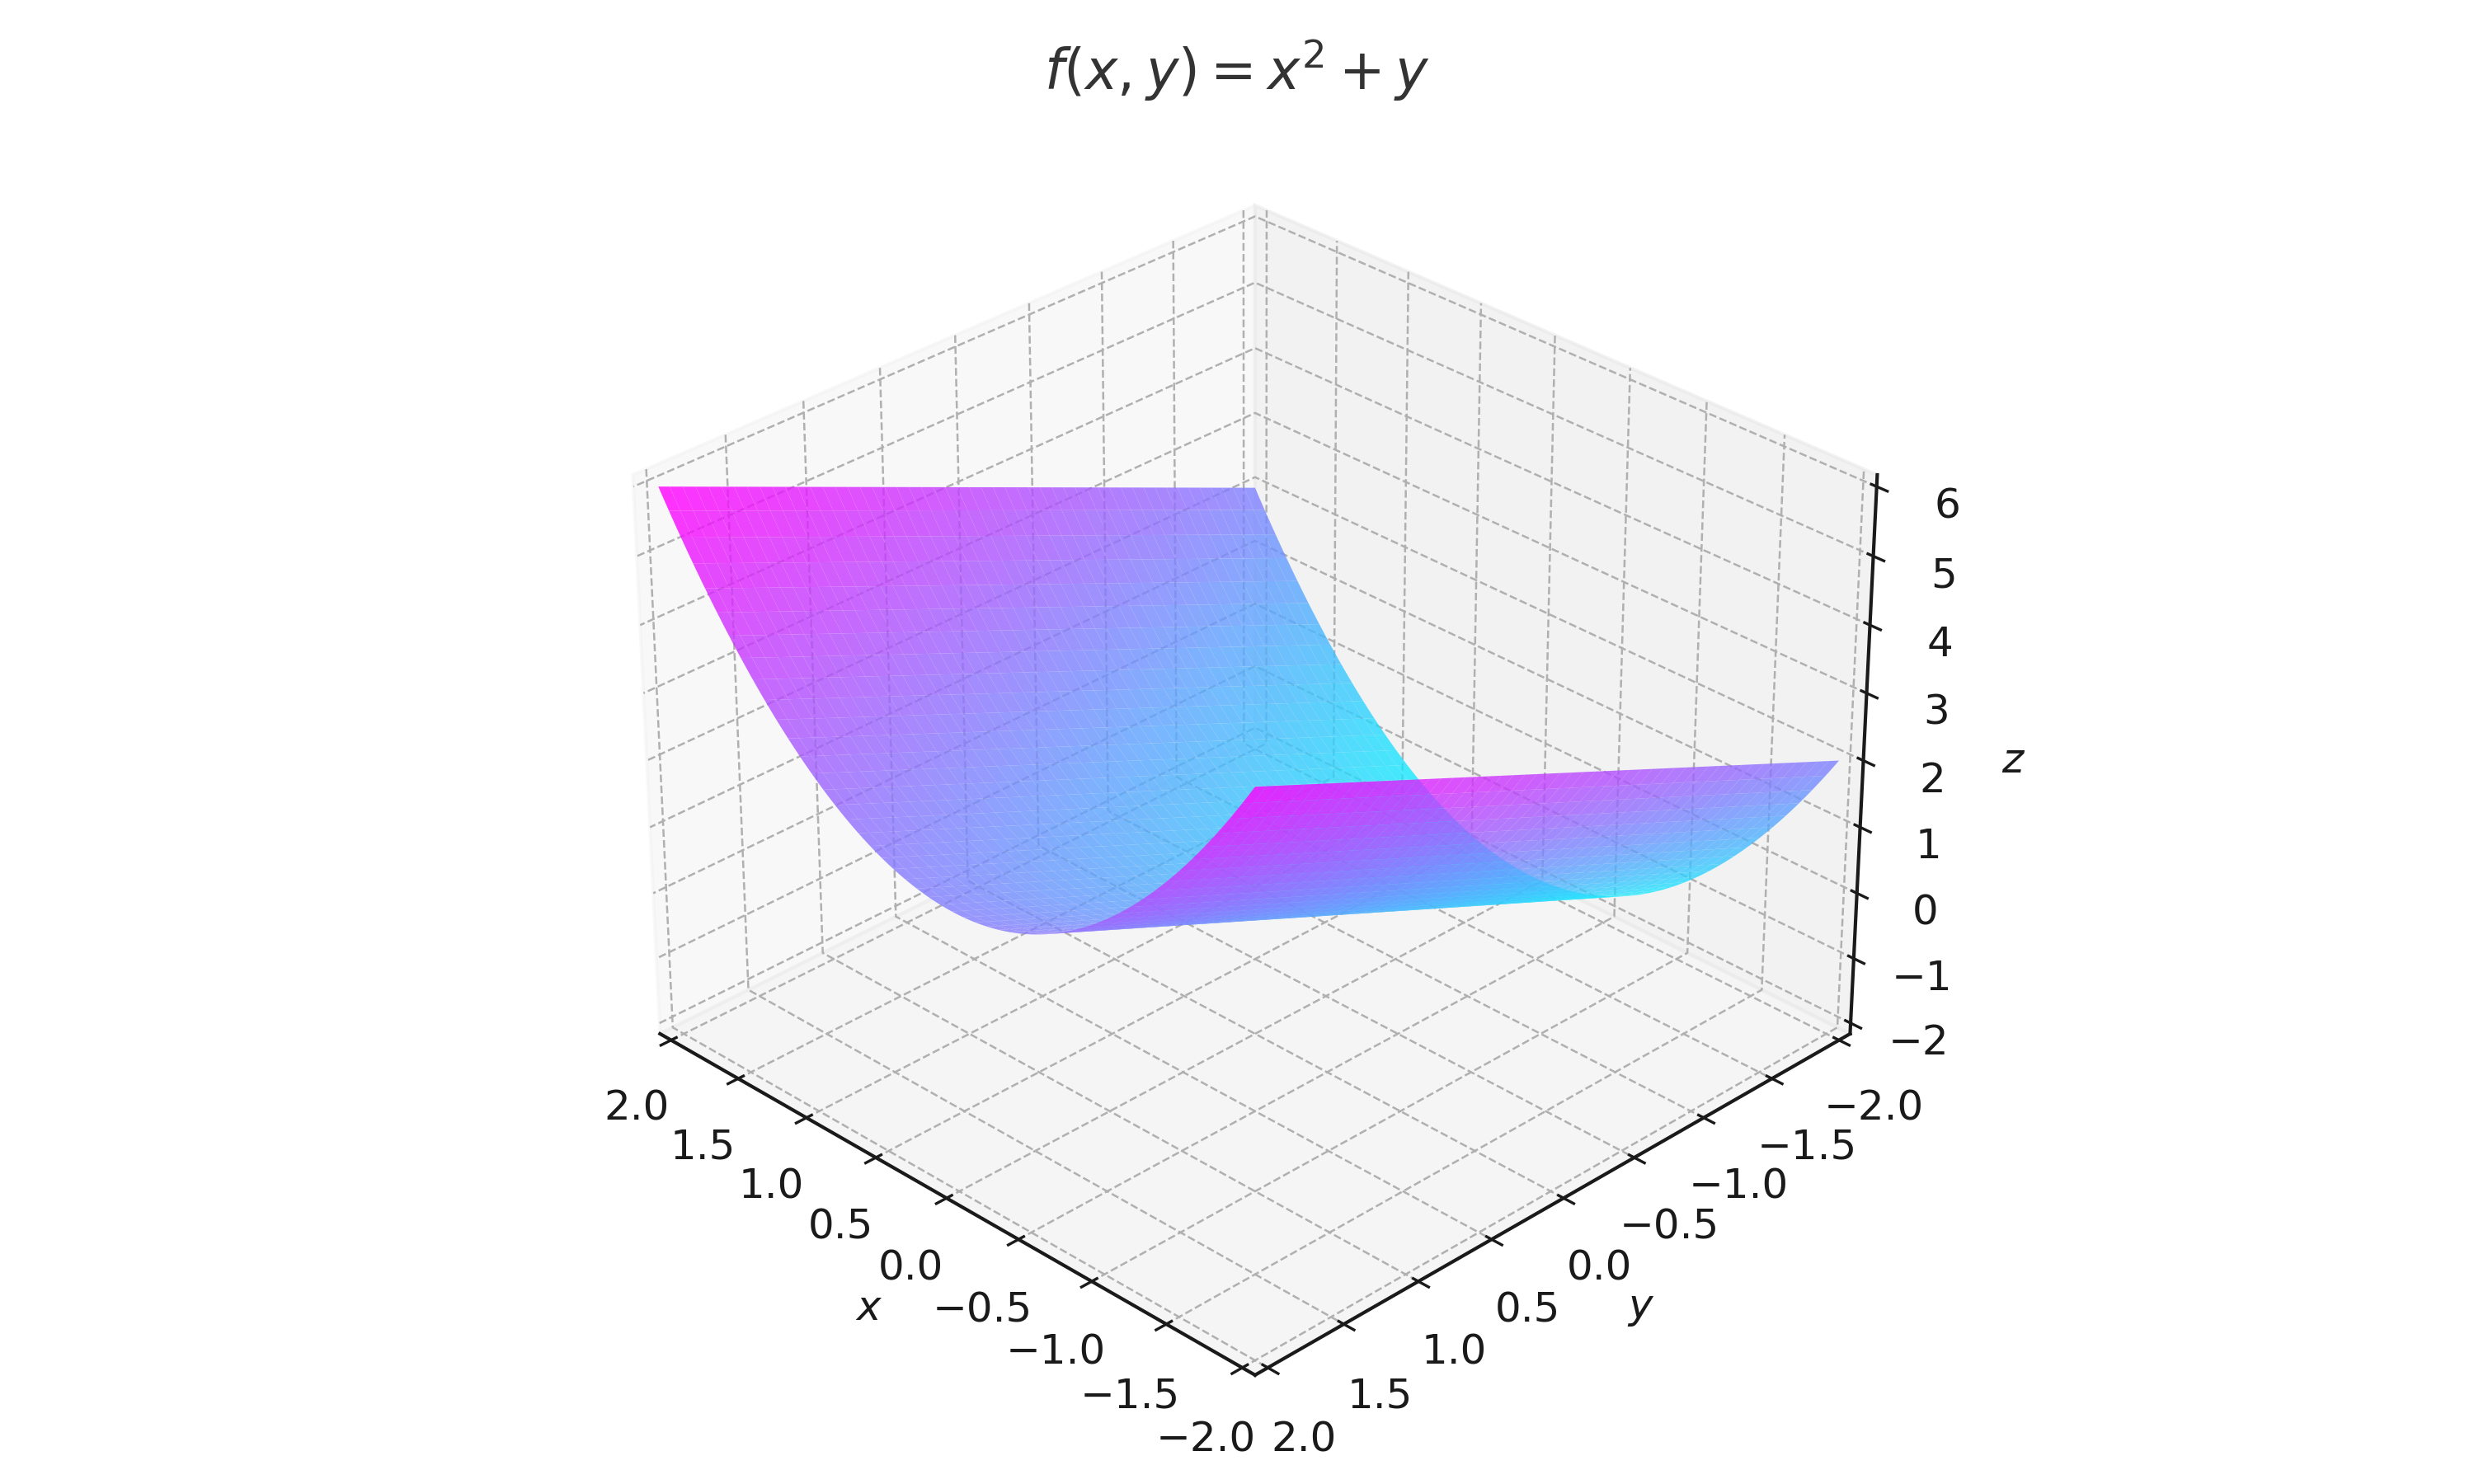
\includegraphics[width=\linewidth]{media/ueb1/graph_f2_labeled.png}
				            \caption*{Graph der Funktion \( f(x, y) \)}
			            \end{subfigure}

			            \caption{Visualisierung von \( f(x, y) = x^2 + y \)}
			            % \begin{subfigure}[t]{0.48\textwidth}
			            %   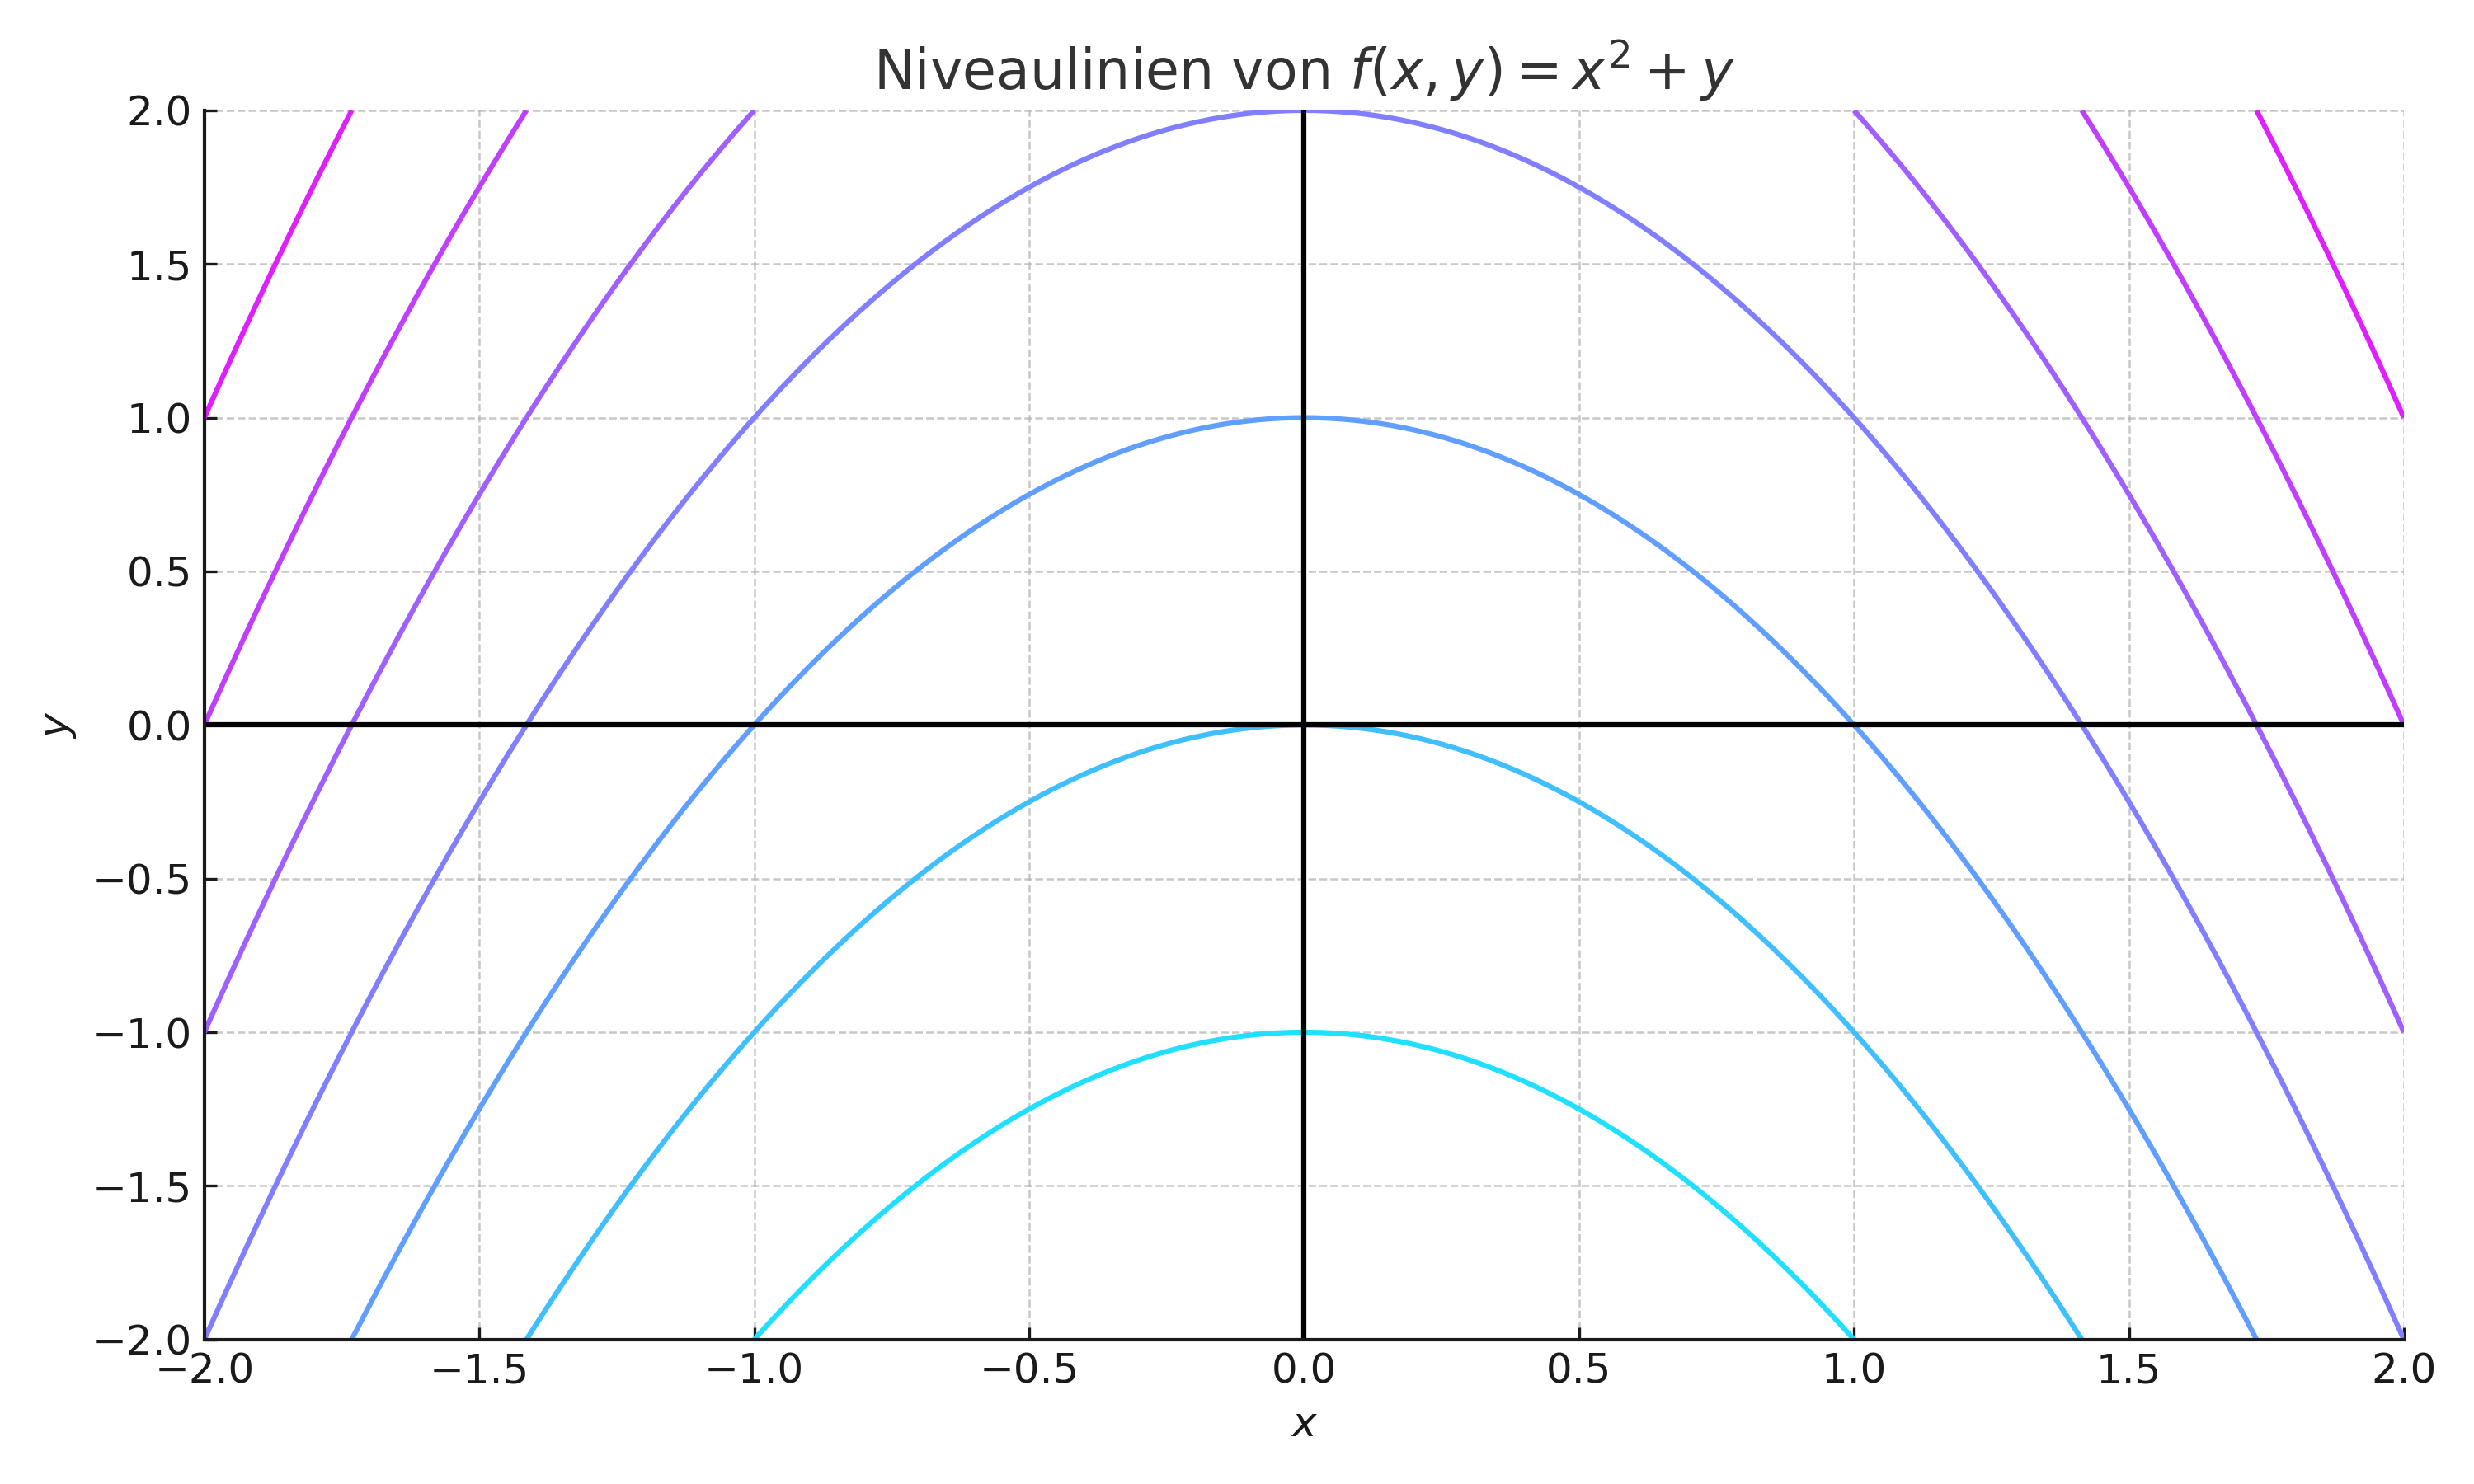
\includegraphics[width=\linewidth]{media/ueb1/niveau_f2_labeled.png}
			            %   \caption{Niveaulinien in der \( xy \)-Ebene}
			            % \end{subfigure}

			            % \vspace{1em}


		            \end{figure}
	      \end{enumerate}
	      \clearpage
	\item Niveaulinien
	      \begin{enumerate}
		      \item

		            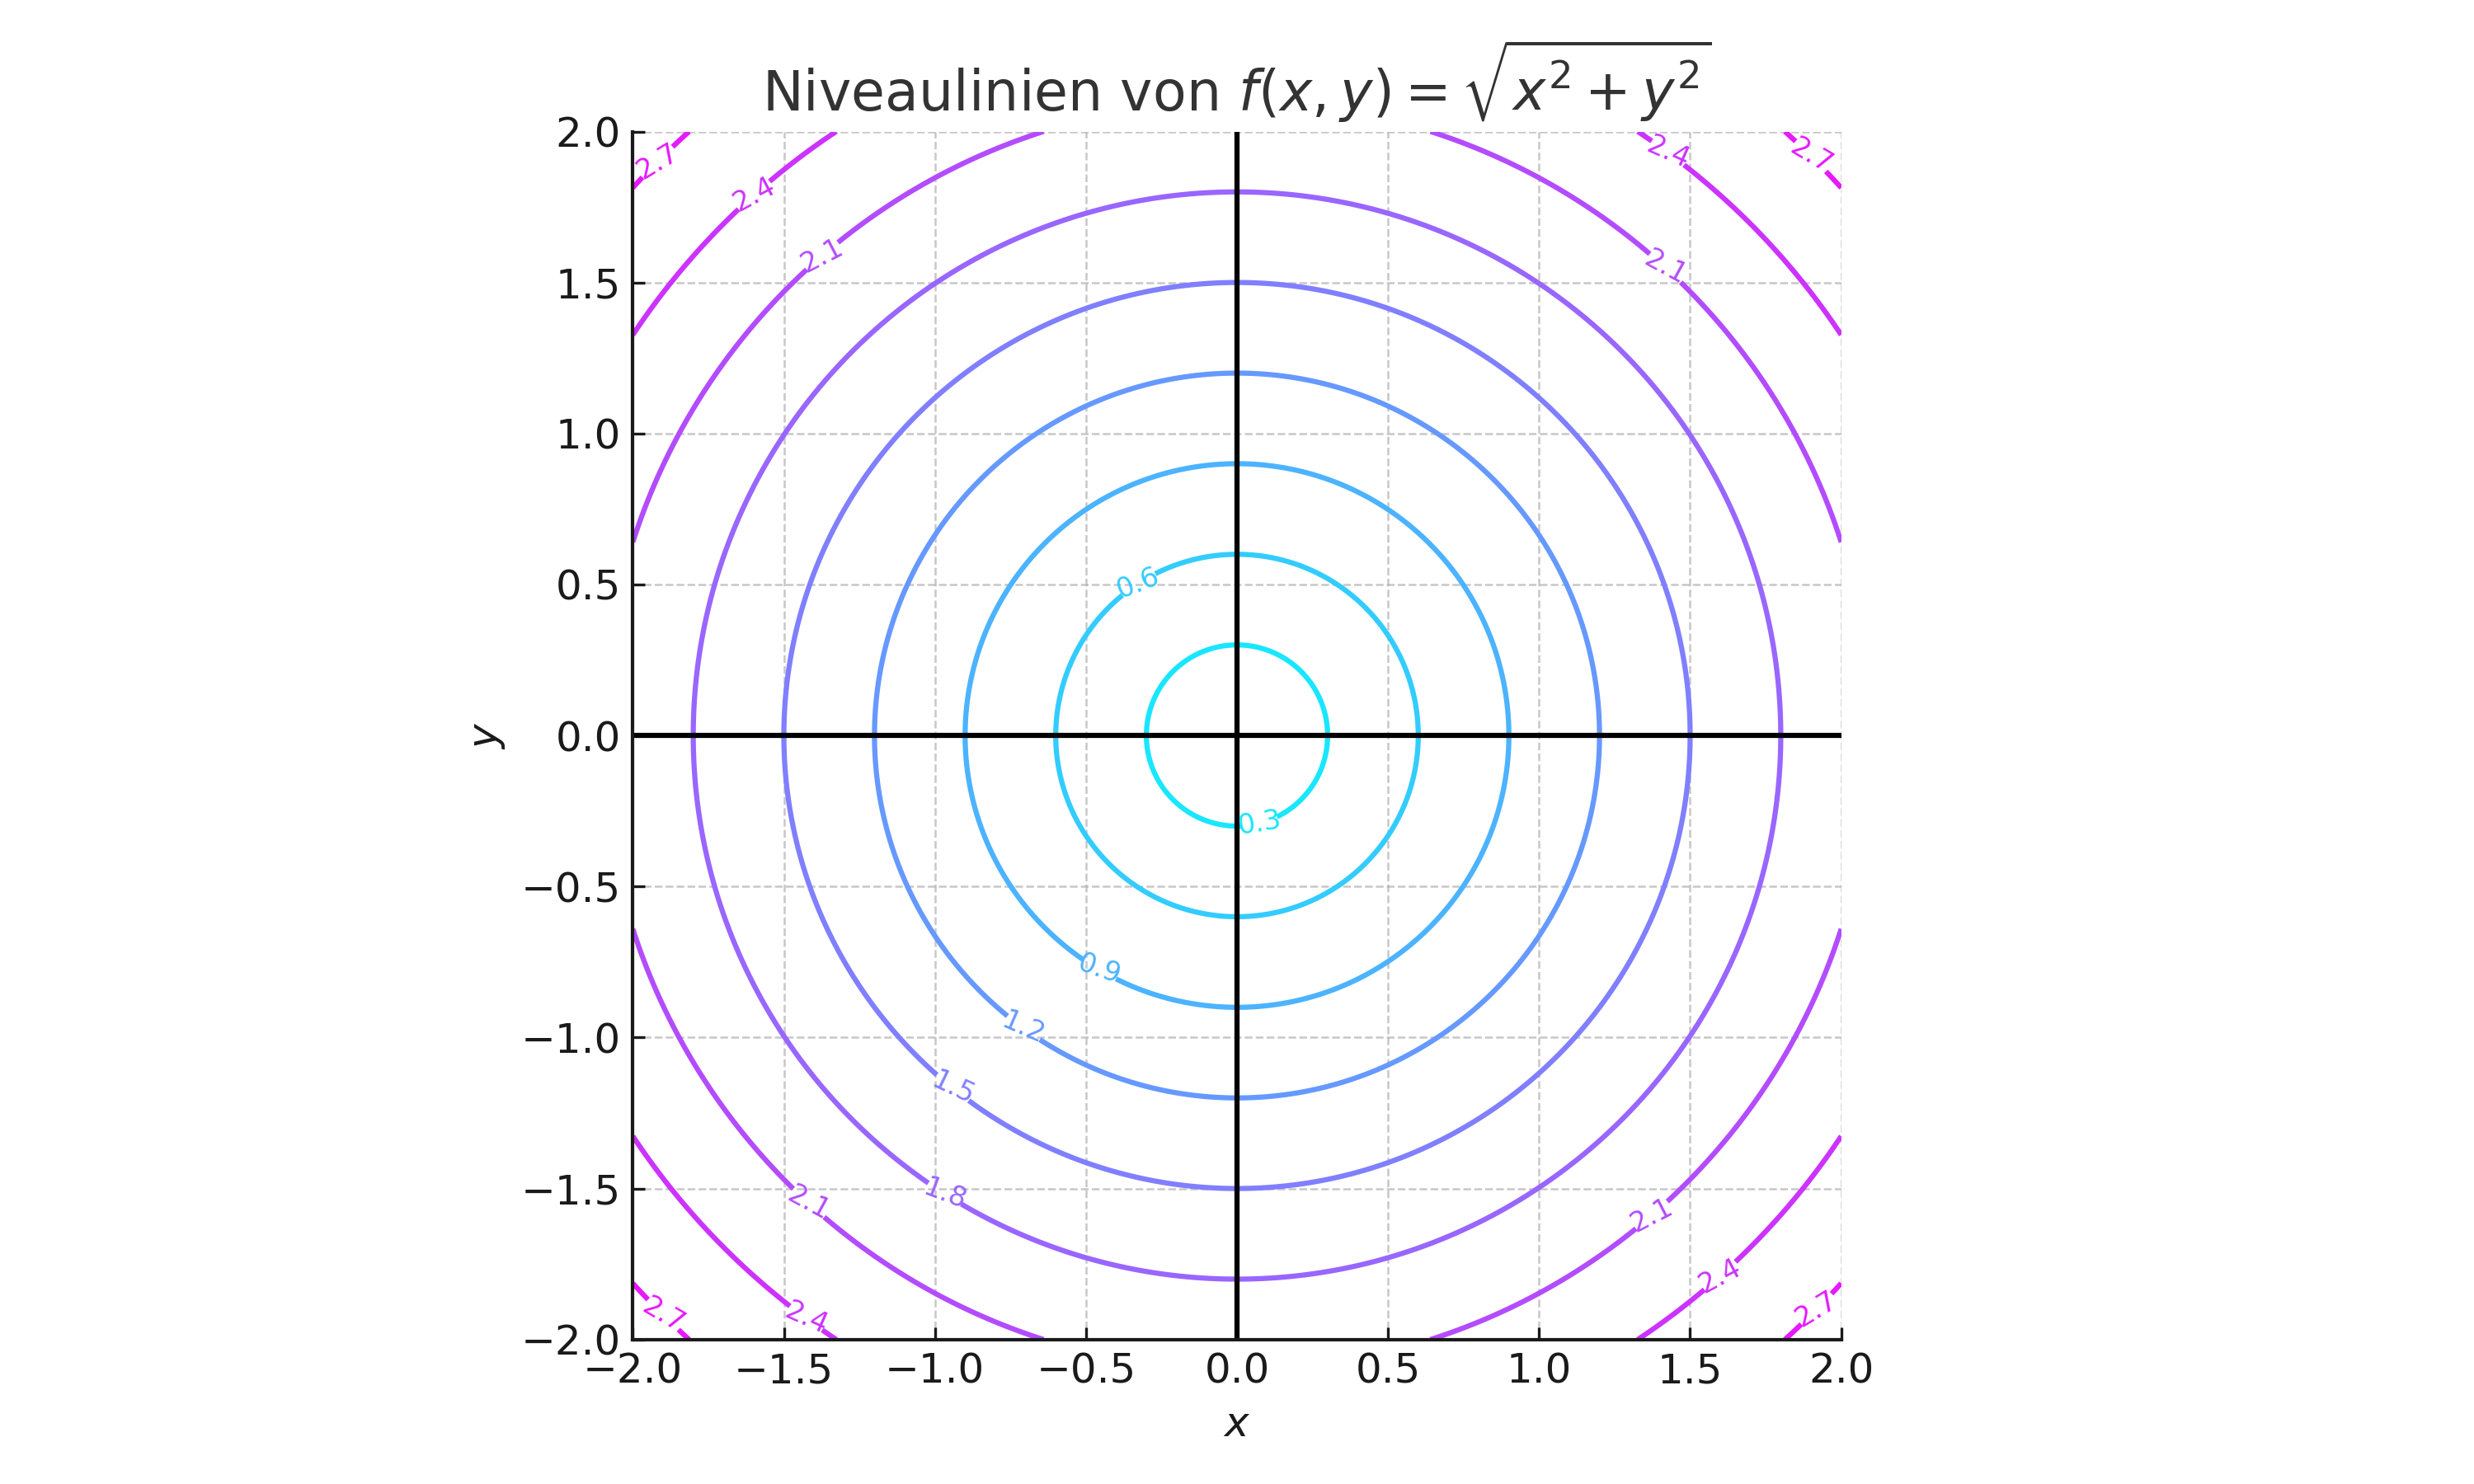
\includegraphics[width = 0.5\textwidth]{media/ueb1/niveau_g2_sqrt_contour.png}
		      \item

		            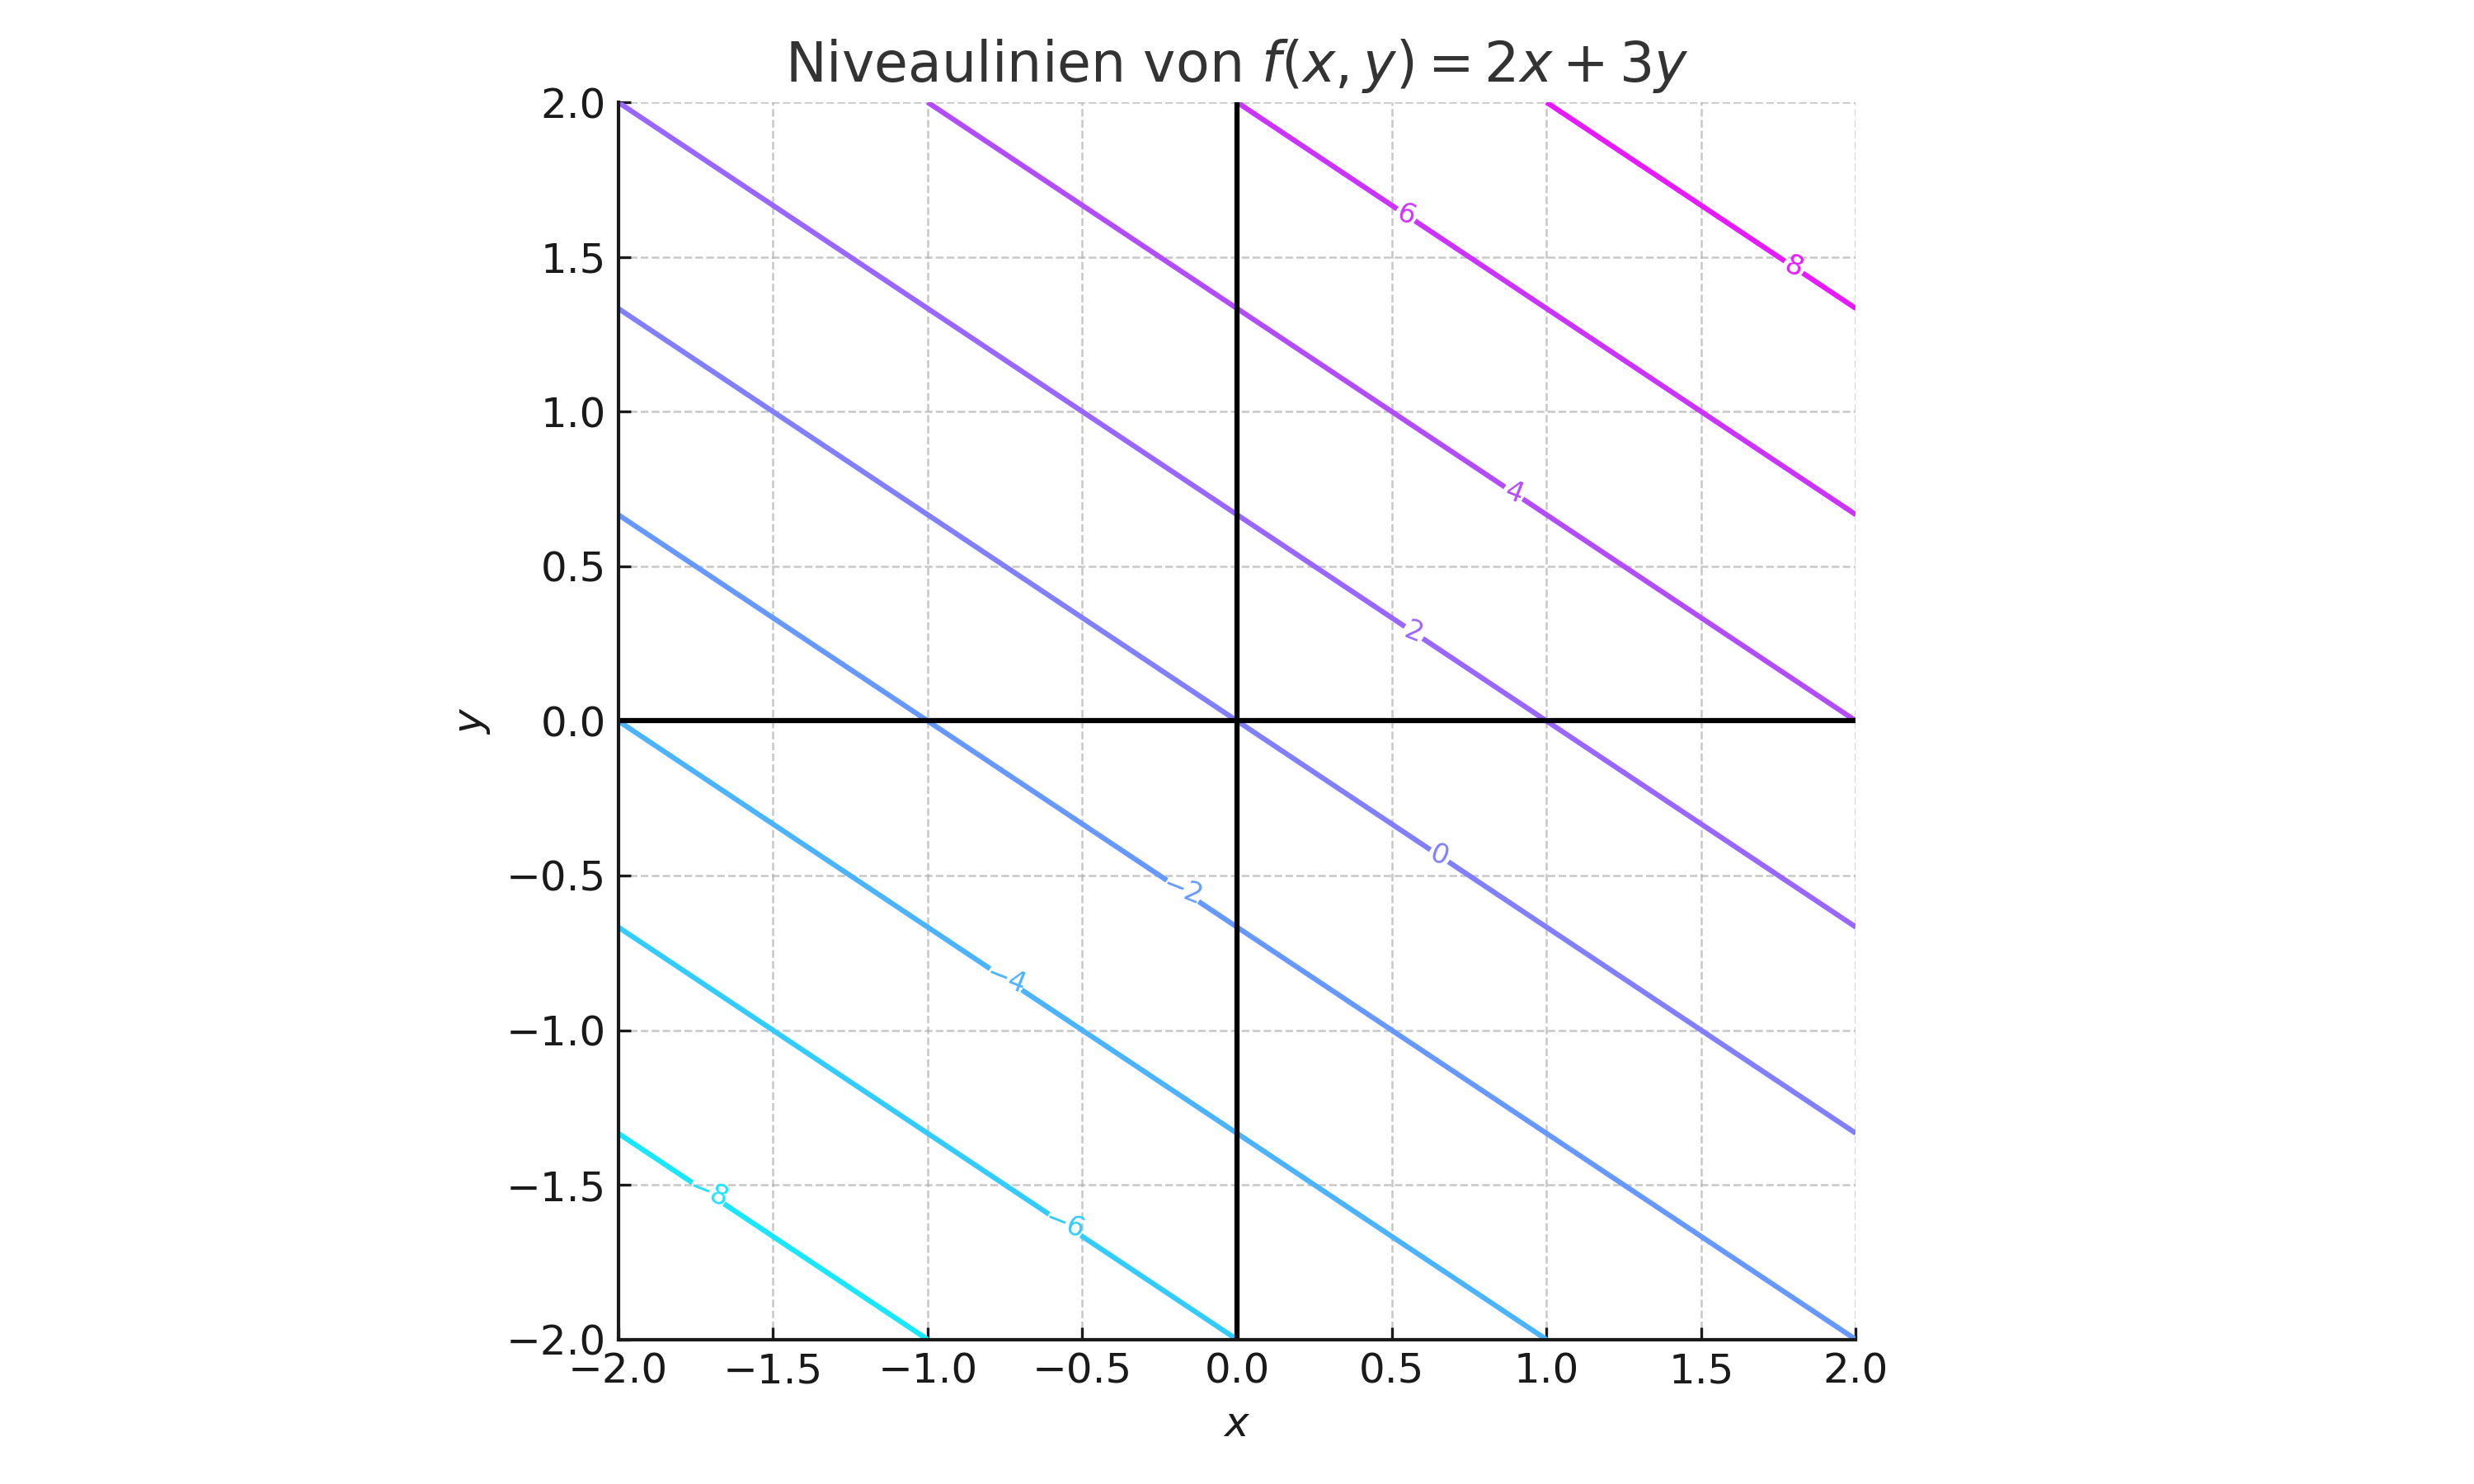
\includegraphics[width = 0.5\textwidth]{media/ueb1/niveau_g3_linear_contour.png}
		      \item

		            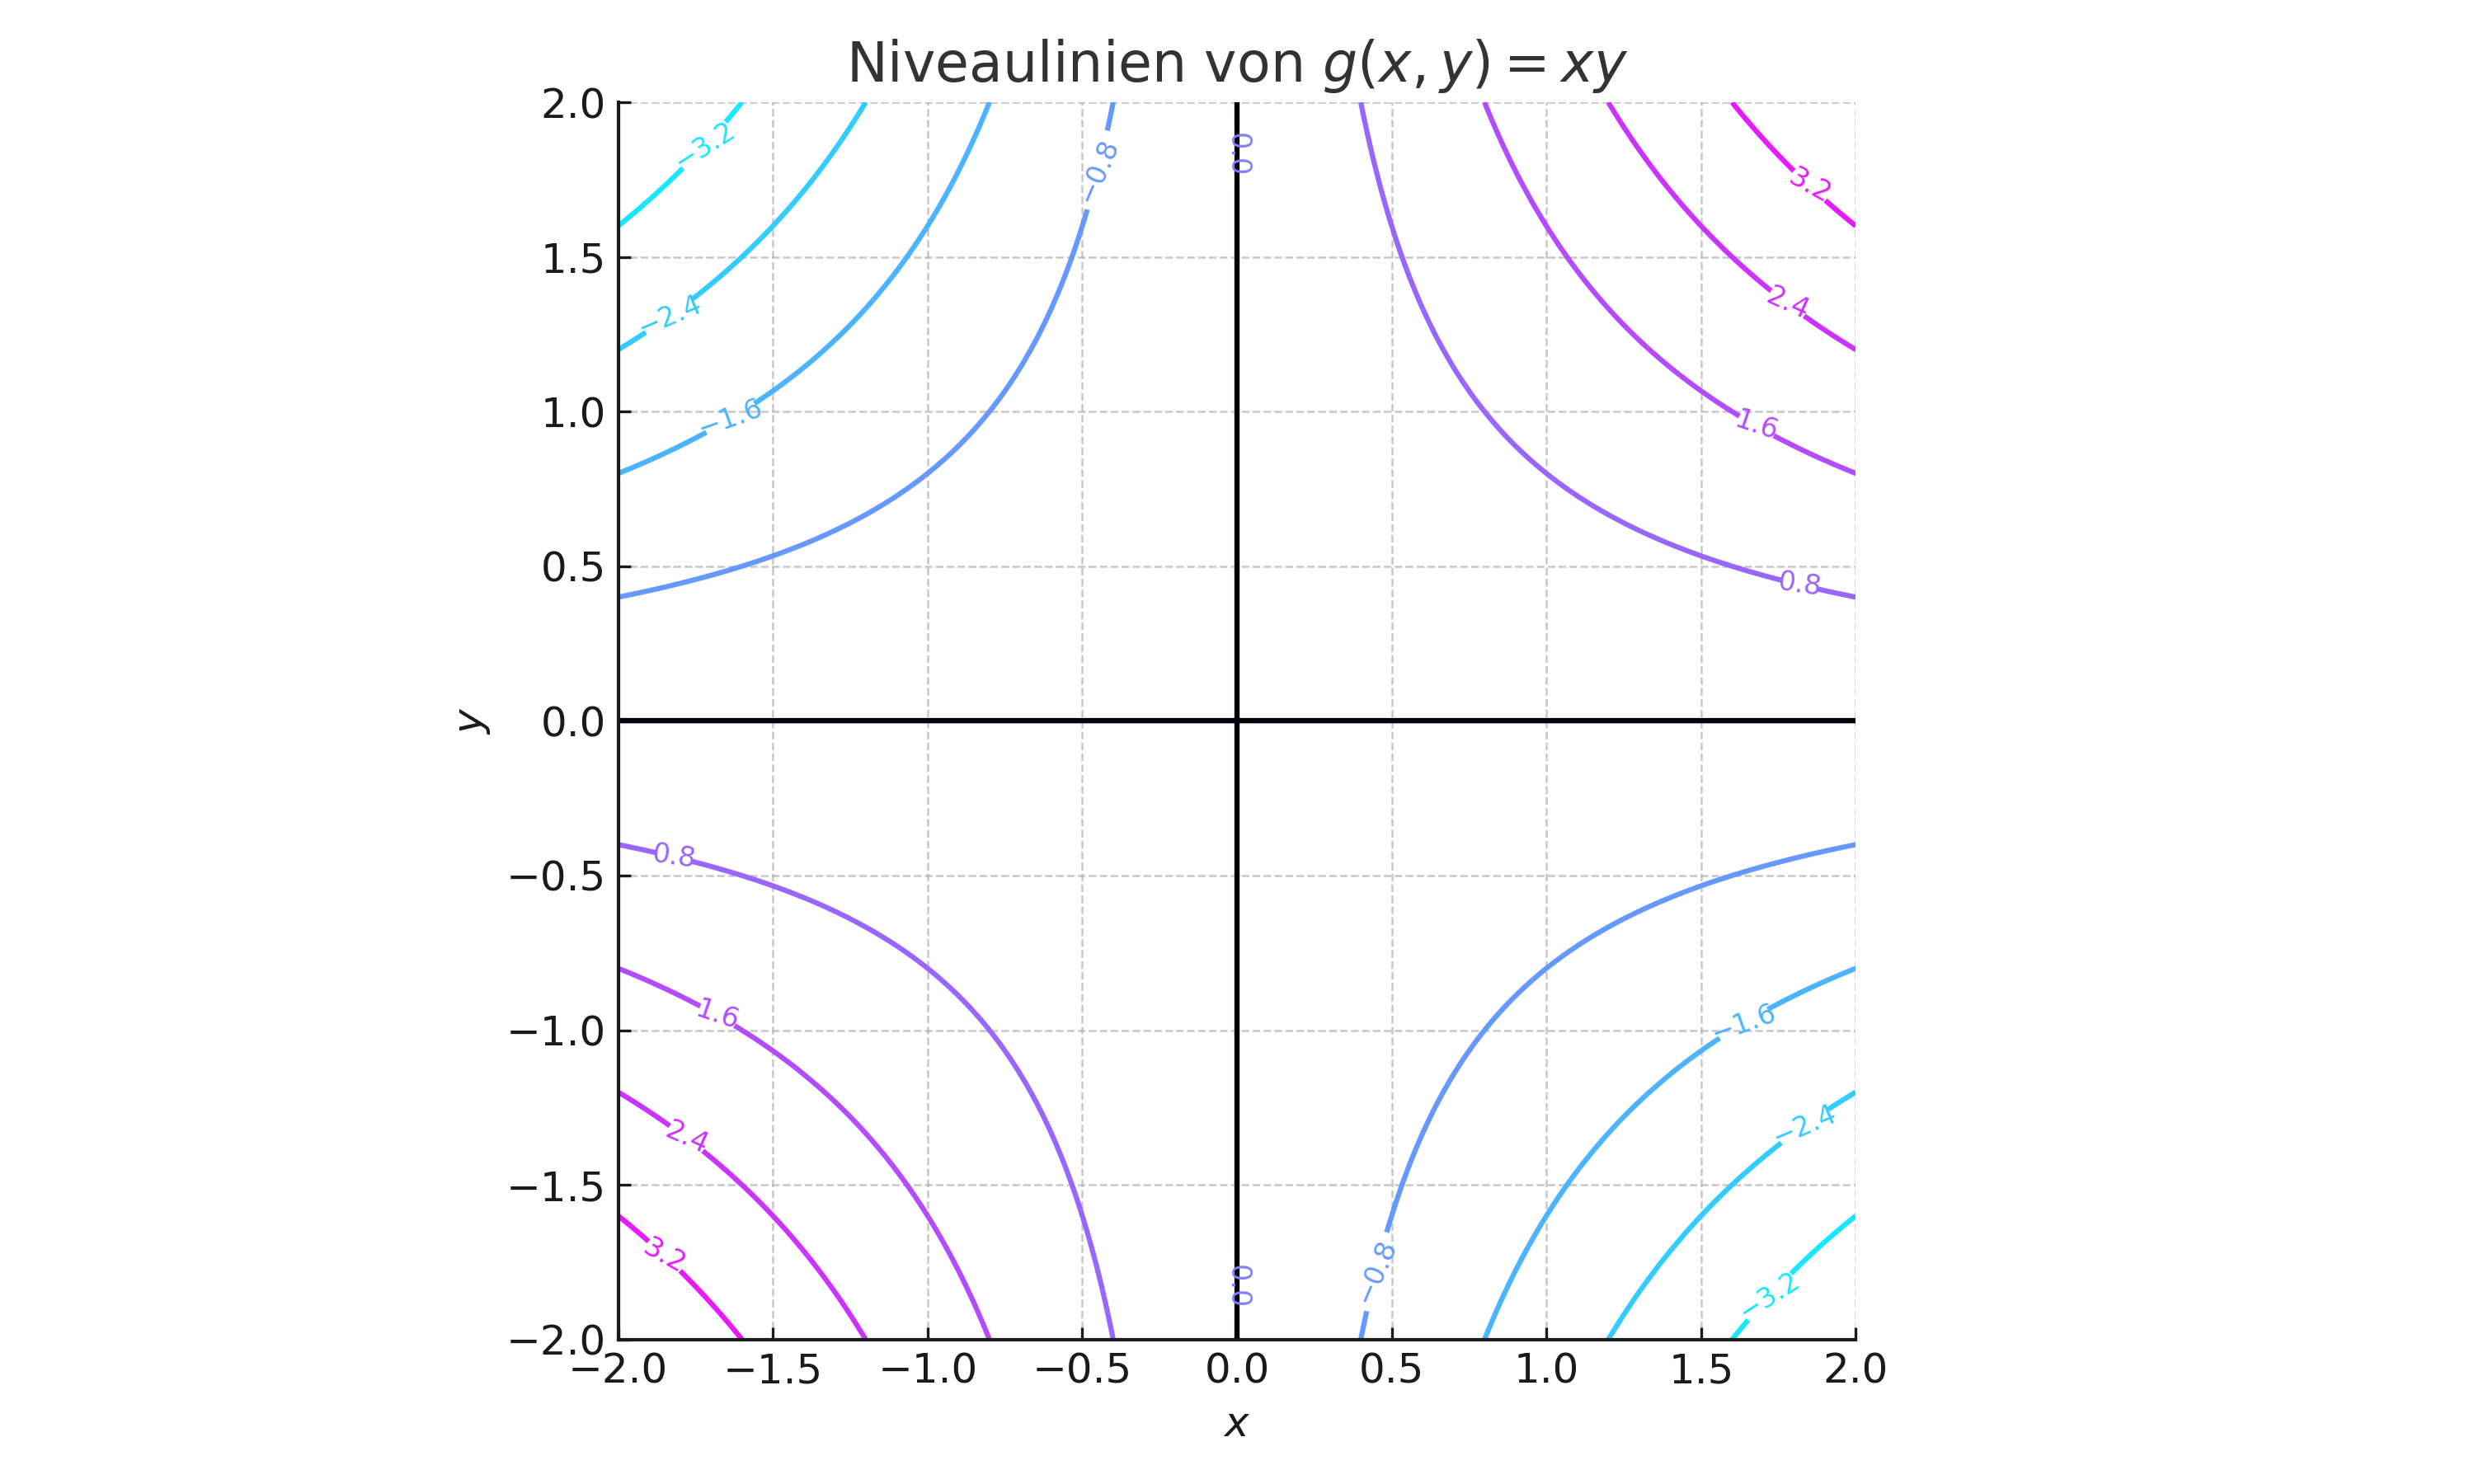
\includegraphics[width = 0.5\textwidth]{media/ueb1/niveau_g1_xy_contour.png}
	      \end{enumerate}
\end{enumerate}